\documentclass[12pt]{article}
\usepackage{authblk}
\usepackage[english]{babel}
\usepackage{threeparttable}
% Bibliography Style
\usepackage[authoryear]{natbib}  % Enables Chicago author-date citations
\bibliographystyle{chicago}
\newcommand{\sym}[1]{\rlap{$^{#1}$}}
\usepackage{soul}
\usepackage{amsmath}
\usepackage{graphicx}   % Required for \resizebox{}
\usepackage[colorlinks=true, allcolors=blue]{hyperref}
\usepackage{ulem} % For \uline command

 \newcommand\citeapos[1]{\citeauthor{#1}'s (\citeyear{#1})} % use apostrofe for references e.g. Lehr's (1990)
\makeatletter
 \def\@mb@citenamelist{cite,citep,citet,citealp,citealt,citeapos} % this will add the custom made command 'citeapos' to the list of newcite commands
 \makeatother
% Margins: 1-inch all around
\usepackage[margin=1in]{geometry}

% Font: Times New Roman (or closest equivalent)
% \usepackage{times}  

% Table & Formatting Packages
\usepackage{threeparttable} % For notes below tables
\usepackage{multirow}
\usepackage{makecell}
\usepackage{array}          % Improved column alignment
\usepackage{siunitx}        % Proper numeric alignment
\usepackage{booktabs}       % Professional table formatting
\usepackage{float}          % Ensures float placement control

% Caption Formatting
\usepackage{caption}   
\captionsetup[table]{
  labelsep = period, % "Table 1."
  justification = centering,
  font = bf, % Bold table caption
  textfont = {bf}
}
\usepackage[table]{xcolor}
% Double spacing for the manuscript
\usepackage{setspace}
% \doublespacing

% Section Formatting
% \usepackage{titlesec}   
% \titleformat{\section}
%   {\large\bfseries}  % Large and bold
%   {\thesection\ \textbar}  % Section number followed by a vertical bar "|"
%   {0.5em}            % Space between "|" and title
%   {\MakeUppercase}   % Convert title to uppercase

\usepackage{xcolor}




\title{\textbf{Game structure obviousness in homegrown preference elicitation}}

\author[1]{Levenson Badio\thanks{Department of Agricultural Economics, Texas A\&M University, College Station, TX  77843 USA, tel:+1-9792407106 e-mail: \href{mailto:levenson.badio@tamu.edu}{levenson.badio@tamu.edu}.}}
\author[1]{Marco A. Palma\thanks{Professor and Director Human Behavior Laboratory, Department of Agricultural Economics, Texas A\&M University, College Station, TX  77843 USA, tel:+1-9798455284 e-mail: \href{mailto:mapalma@tamu.edu}{mapalma@tamu.edu}.}}
\author[2]{Andreas C. Drichoutis\thanks{Professor, Department of Agricultural Economics \& Rural Development, School of Applied Economics and Social Sciences, Agricultural University of Athens, Iera Odos 75, 11855, Greece, e-mail: \href{mailto:adrihout@aua.gr}{adrihout@aua.gr}.}}
\author[1]{Samuel Zapata\thanks{Associate Professor, Department of Agricultural Economics, Texas A\&M University, McAllen, Texas, USA, tel: +1-956-9685585 e-mail: \href{samuel.zapata@ag.tamu.edu}{samuel.zapata@ag.tamu.edu}.}}
\author[1]{Rodolfo M. Nayga, Jr.\thanks{Professor, Department of Agricultural Economics, Texas A\&M University, College Station, TX  77843 USA, and Adjunct Professor, Korea University; tel:+1-9798452116 e-mail: \href{mailto:rnayga@tamu.edu}{rnayga@tamu.edu}.}}

\affil[1]{Texas A\&M University}
\affil[2]{Agricultural University of Athens} 
\date{}

\begin{document}


\maketitle
 \onehalfspacing

\begin{abstract}
\noindent The Becker-Degroot-Marschak (BDM) mechanism is widely used in experimental valuation research because of its theoretical incentive compatibility and implementation simplicity. However, recent work challenges BDM mechanism's ability to match outcomes that closely represent its theoretical predictions in induced value (IV) settings. The Game Structure Obvious (GSO) mechanism is a new method that has shown promising results in aligning IV theoretical predictions with empirical findings. The GSO mechanism however has not been tested in homegrown settings, which are particularly important in environmental and market valuations for understanding demand for new or unfamiliar products. In this study we test the BDM and the GSO mechanisms in an online homegrown experiment eliciting consumers' preference for oranges from trees treated with antibiotics, and compare the valuation outcomes in real and hypothetical treatments. This research question is important to identify the optimal tools for measuring food and resource valuations with incentives reflecting actual market values. Our findings reveal a counterintuitive methodological insight: while the GSO is perceived as simpler and more intuitive than the BDM mechanism in all treatments, the GSO mechanism induces significant hypothetical bias in early decision rounds, while the BDM mechanism does not. Under real incentives, both mechanisms yield equivalent valuations, but under hypothetical conditions GSO produces  higher valuations than BDM . The bias stems entirely from selective inattention--GSO participants spend less deliberation time in hypothetical settings, and when controlling for deliberation time, hypothetical bias disappears by rounds 2-3. GSO demonstrates substantial learning effects with hypothetical bias declining 67\% by Round 3, while BDM shows no learning patterns.

\textbf{Keywords:} Strategy-proof, BDM, GSO, hypothetical bias, citrus greening, oranges. 
	
\textbf{JEL codes:} C90, C91, D44, D80
 
 \textbf{AEA RCT Registry:} \#0014656
 
 \end{abstract}


\onehalfspacing
\section{Introduction}
Obtaining accurate estimates of individual valuations for products and services is crucial for guiding policy recommendations and driving product development innovations. Experimental auctions and auction-like mechanisms are prominently used tools in valuation studies \citep{lusk2007experimental,canavari2019run}. However, reliably uncovering true preferences remains a persistent challenge--even in cases where the good in question has a simple, fixed, and objectively measurable value \citep{drichoutis2022game, cason_misconceptions_2014}. One commonly used method for eliciting preferences--especially in settings where direct interaction with participants is limited--is the Becker-DeGroot-Marschak (BDM) mechanism,  favored for its simplicity and theoretical incentive compatibility \citep{mamadehussene2023reliability, azrieli2018incentives}. The BDM mechanism is widely used in online studies to measure product valuations, beliefs, subjective probabilities, and trust  \citep{mamadehussene2023reliability, ahles_testing_2024, burdea2022online}. In this mechanism, participants submit a bid for a good, knowing that a price is randomly drawn from a predetermined range. If the participant's bid is equal to or exceeds the drawn price, they purchase the item at that price. Otherwise, they do not receive the item \citep{becker_measuring_1964}.

Despite its theoretical appeal, the BDM mechanism has shortcomings. 
\citet{cason_misconceptions_2014} highlighted key pitfalls of the BDM mechanism within a simple induced value framework, where participants were asked to provide their willingness to accept (WTA) for a card with a known fixed objective value of \$2. This study directly challenges the theoretical incentive compatibility of the BDM mechanism by showcasing that only 16.7\% of participants bid within 5\% of the actual value of \$2.\footnote{However, bidding accuracy (within the \$2) increases with learning and roughly doubles by the second round of bidding \cite{cason_misconceptions_2014}.} This issue is not unique to the BDM mechanism; \citet{DrichoutisEtAl2024incentives} report similar findings to \citet{cason_misconceptions_2014} with only 24.7\% of bidders submitting bids within 5\% of the induced value in the BDM mechanism, while second-price auctions show only modest improvements to 27.4\%. Given the consistent failure of participants to bid accurately even in simple, controlled settings with objectively defined values, the reliability of these mechanisms as tools for eliciting true market preferences warrants serious scrutiny.

The persistent failure of existing elicitation mechanisms to induce truthful bidding, even in settings where weakly dominant strategies should be obvious, has motivated the development of new strategy-proof methods designed to make optimal choices more apparent to participants \citep{li_obviously_2017, pycia_theory_2023}. Strategy-proof mechanisms are those in which participants have no incentive to misrepresent their true preferences, as doing so offers no benefit. Among these, the Game Structure Obvious (GSO) mechanism has emerged as a novel and increasingly prominent tool. It is recognized both for being strategy-proof and for making weakly dominant strategies more transparent and intuitive to participants \citep{chakraborty_future_2025}. 

In the context of homegrown valuation, the GSO mechanism functions as a multiple price list in which participants progressively choose, at each step, whether to purchase or decline an item at a given price \citep{yu2021multiple, herberich2012digging, jack2022multiple}.  The price starts at a fixed level and increases by a constant increment until it reaches a terminal value randomly determined at the outset. We argue that comparing GSO with the BDM mechanism in a homegrown setting is essential for two reasons. First, in induced value settings, the GSO  has demonstrated significantly higher bidding rates closer to theoretical predictions--between 43\% and 58\%--compared to the BDM, which achieves a bid accuracy rate of around 15\% \citep{chakraborty_future_2025}. However, it is unclear whether these results transfer verbatim to a homegrown setting. Secondly, since the GSO mechanism has not yet been empirically applied in homegrown valuation studies, its reliability in settings involving hypothetical scenarios remains an open question.

Unlike induced value studies, homegrown valuation involves items whose value is heterogeneous and not objectively defined. Consequently, we focus on which elicitation method produces valuations further away from purely hypothetical values.  This topic is important to address given that market and resource valuations are more complex and often involve the evaluation of multiple attributes and information.  Therefore, evaluating the performance of the GSO and BDM mechanisms under both hypothetical and incentivized conditions is critical to establish meaningful benchmarks for future use. 

To assess their performance in homegrown value settings, we implemented an online experiment with a sample representative of the U.S. population in order to test the performance of the GSO and BDM mechanisms under real and hypothetical incentives; the hypothetical treatments served as baseline. As a case study, we elicited consumers' willingness to pay (WTP) for fresh oranges from trees treated with trunk-injected antibiotics for Huanglongbing (HLB) and conventionally grown oranges. This application is relevant to the citrus industry that seeks to adopt economically and logistically feasible methods to control the disease that threatens to decimate the industry while ensuring consumer acceptance (see Appendix \ref{AppedixOrange} for more information). 

Our findings highlight several stylized facts. First, participants perceive the GSO mechanism as less complex than the BDM mechanism, aligning with its intended design to make optimal strategies more transparent. Interestingly, while we find no evidence of hypothetical bias under the BDM mechanism, we observe clear evidence of such bias under the GSO mechanism. 
The source of this paradox lies in differential attention allocation. Our analysis demonstrates that GSO's hypothetical bias stems entirely from selective inattention: participants spend significantly less deliberation time in hypothetical settings, and when we control for this attention differential, hypothetical bias disappears by rounds 2-3. This reveals that GSO's apparent weakness is not inherent to the mechanism but rather reflects how participants engage when stakes are absent.
Critically, GSO demonstrates substantial learning capabilities that BDM lacks. Hypothetical bias declines by 67\% from Round 1 to Round 3 in GSO, while BDM exhibits no learning patterns across rounds. When controlling for attention, GSO's learning eliminates bias entirely in later rounds. Under real incentives, both mechanisms perform equivalently, confirming that the issue is not GSO's fundamental design but participants' strategic attention allocation.
These results provide three key methodological insights for homegrown preference elicitation. First, mechanism transparency and bias mitigation follow a non-monotonic relationship--excessive obviousness without real stakes may paradoxically encourage shallow processing. Second, the superiority of GSO documented in induced-value settings does not transfer directly to homegrown contexts where attention allocation becomes crucial. Third, GSO's learning advantages suggest it may be particularly valuable in multi-round experimental designs where participants can discover optimal strategies, provided sufficient attention is maintained through appropriate incentive structures.


We make several important contributions to the preference elicitation and experimental economics literature. First, we extend the growing literature on strategy-proof mechanisms by providing the first systematic evaluation of the GSO mechanism in homegrown valuation contexts, where true values are subjective and unknown \citep{li_obviously_2017, pycia_theory_2023, chakraborty_future_2025}. While previous research has demonstrated GSO's superiority in induced value settings with known objective values, our findings reveal that these advantages do not transfer directly to real-world valuation scenarios involving consumer preferences. Second, our work contributes to the hypothetical bias literature \citep{penn2018understanding, cummings1999unbiased, loomis_whats_2011, fang_use_2021, list2001explicit, grebitus2013explaining} where we uncover a counterintuitive finding: the GSO mechanism, despite being game strategy obvious and superior to the BDM mechanism in IV settings, exhibits significant hypothetical bias while the BDM mechanism does not (at least not in this study). This suggests that the relationship between mechanism complexity and bias mitigation can be non-monotonic and context-dependent. Third, we advance understanding of learning effects in preference elicitation \citep{drichoutis2011role, canavari2019run} by demonstrating that the GSO mechanism facilitates dynamic learning processes that reduce hypothetical bias over successive rounds, while the BDM mechanism shows no such learning patterns. This finding has important implications for multi-round experimental designs and suggests that the 
GSO mechanism may be particularly valuable in educational or repeated-interaction contexts. Finally, our study provides methodological guidance for applied consumer research by showing that elicitation method choice can substantially affect estimated valuations, particularly under hypothetical conditions, reinforcing the importance of careful mechanism selection in valuation studies\citep{miller2011should, schmidt2020accurately}.

Our paper proceeds as follows. Section~\ref{Experiment} describes the experimental design, procedures and data collection, Section~\ref{Econometric} presents the empirical analytical methods, Section~\ref{Results} shows the results, and conclude in Section ~\ref{Conclusion}.

\section{Experimental methods}
\label{Experiment}
This section outlines the experimental protocol, including the design, procedures, and data collection strategies used to investigate our primary research question. The subsections that follow describe we describe the experimental protocol that we followed, a description of the methods, procedures and data collected to address our main research question. 

\subsection{Experimental Design}
Our study employed a $2\times2$ between-subject design that varied across two dimensions: elicitation method (BDM vs. GSO mechanism) and incentives (Hypothetical vs. Real incentives). Hence, subjects were randomly assigned to one of the four treatment groups. In the hypothetical incentives treatment, subjects were explicitly informed that none of the described payoffs or potential purchases were real or were actually going to take place and they would only receive a participation fee. In the real incentives treatment, we implemented a Between-Subject Random Incentivized Scheme (BRIS) with a 10\% realization probability \citep{ahles_testing_2024}. On top to their participation fee, each participant was endowed with \$6 that they could potentially use to buy a 3.2 pound bag of oranges during the experiment with the understanding that any leftover money would be added to their bonus payment. Subjects submitted bids in three consecutive rounds, and at each round they could bid for a bag of conventional oranges and a bag of oranges from trees treated with antibiotics. Participants were aware that at the end of the experiment one round and one product would be randomly drawn as binding and any transactions regarding that product and round would be realized.\footnote{ However, for the hypothetical treatments, participants were explicitly informed of the hypothetical nature of the endowment and decisions.}  

The elicitation task was carried out in three rounds to assess the role of learning \citep{corrigan2008testing, drichoutis2011role} in value elicitation. The first two rounds of bidding were exactly the same (i.e., no new information was added between the rounds) and with only basic information about the types of oranges as normally presented in real markets. Before the third round, we introduced an information treatment video that informed subjects about the impact of HLB on the US citrus industry.\footnote{Participants watched a 51 seconds \href{https://www.youtube.com/watch?v=_AqMBjB0ChM}{video} containing objective information about the impact of HLB on the US citrus industry, the livelihood of farmers, and its potential risk to human health and the environment. The information script was revised by agricultural scientists to ensure the accuracy and veracity of the information. This design allows us to measure the impact of information provision on WTP for oranges from antibiotic-treated orange trees relative to conventional oranges.} In both the BDM and the GSO mechanism treatments, the prices were randomly drawn from a uniform distribution of [\$0, \$6] with increments of \$0.20.\footnote{We chose the 20 cents increments to balance between bid precision, time and cognitive load, following the literature using an increment representing 3.33\% of the endowment leading to a maximum of 31 decisions per round \citep{li_obviously_2017, chakraborty_future_2025}. The upper bound of the range was chosen based on the actual maximum value of the orange prices in the market at the time of the study plus a price premium of 40\% higher than the market price for those willing to pay a premium for oranges from antibiotic-treated orange trees.}

In the BDM mechanism treatment, subjects had to use a slider to select their bid. If their bid for a 3.2 pound bag of oranges was greater than or equal to the randomly drawn price, they would buy the product at the randomly drawn price, otherwise, they would not buy the product and would keep their endowment.

In the GSO mechanism treatments, at the start of each round, an `Offer Price' appeared on the screen that was subsequently increased in fixed increments of \$0.20 after each decision they made. %This increment was selected to strike a balance between generating realistic market price variation and minimizing decision fatigue. Consistent with the literature, the increment corresponds to approximately 3.3\% of the maximum possible value, resulting in a maximum of 31 increments per round \citep{li_obviously_2017, chakraborty_future_2025, brown_is_2023}. 
The offer price for the first screen was set to \$0. The process of increasing the offer price continued until it reached a randomly drawn `market price', which was unknown to participants. The random price was independently drawn for each round from a uniform distribution between \$0 and \$6 and was different between subjects, rounds and treatments. When the offer price matched the randomly drawn price, the round automatically ended.\footnote{See Figure~\ref{fig:Appendix_GSO_game} in the Appendix for an illustration and a link to a video capture of how this dynamic process looked like.} 



One characteristic of the GSO mechanism is that it does not prevent multiple switching behavior (MSB). Specifically, individuals who may initially decide not to purchase at a given (low) price may attempt to buy at a higher price in subsequent rounds. To reduce MSB due to accidental click or lack of attention, we implemented a soft nudge consisting of a warning about MSB, reminding subjects of the last price they chose not to buy and with the option of changing their inconsistent choice \citep{yu2021multiple}.\footnote{Participants retained full freedom to make choices as they wished. To address potential input errors (e.g., accidental clicks), a confirmation prompt was displayed whenever a participant switched from opting to buy to not buying: ``You are deciding not to buy at this price. Do you want to confirm it?''} 
This intervention was designed to reduce MSB caused by inattention. Our main analysis does not exclude subjects that exhibited MSB in the GSO treatment, as these participants may genuinely prefer randomization \citep{agranov2017stochastic}. However, we report results excluding these participants as a robustness check. The results remain robust compared to the main analysis.
    
\subsection{Experimental Procedures}
The experiment was programmed in Qualtrics and the study protocol was approved %by the Institutional Review Board (IRB) at \hl{blind if submitting to AJAE} Texas A\&M University (approval number: STUDY2024-1002). Our study was
and pre-registered with the AEA's RCT registry.
\iffalse
(\href{https://www.socialscienceregistry.org/trials/14656}{AEARCTR-0014656
}). 
\fi
A large representative sample of 2,295 participants were recruited through Forthright Access, an online research company that handles their own recruitment through a variety of direct advertising channels. Of these, 1,111 subjects either declined, failed to meet the screening criteria or the attention checks. This resulted in a final sample of 1,184 participants with complete responses. The data were collected in December 2024. To be eligible, participants had to be at least 18 years old and purchase and eat citrus at least once a month. 
Each participant received a base participation fee of \$2 for completing the study. The study started with participants receiving treatment-specific instructions, followed by comprehension questions. In the real incentivized treatment, participants were informed that they would complete three rounds of elicitation tasks and that one product from a randomly chosen round would be randomly chosen for realization. 

After completing the main bidding task, participants responded to a post-experiment survey to measure perceived complexity and choice certainty.\footnote{We measure perceived complexity by asking how complex they found the valuation task and choice certainty by asking how frequently they felt unsure or inclined to revise their valuations.} For the real incentivized treatments, a random number determined the realization with 10\% probability.  If selected, the winner would receive any remaining funds from their endowment and was asked to voluntarily provide a shipping address to deliver (free of charge) the oranges via priority mail. A separate link was provided to enter the mailing address information to preserve anonymity. A total of 108 (8.7\%) participants were selected for payment, including 27 subjects to whom we shipped bag of oranges. The rest were non-buyers who just received their endowment of \$6 on top of their participation fee. 
%Among the 45 buyers, 36 provided a mailing address and were subsequently shipped the oranges; they also received any remaining balance from their endowment.

% \subsection{Data}


\section{Econometric analysis}
\label{Econometric}
Having established our experimental protocol, we now turn to the econometric analysis that will test our hypotheses about relative mechanism performance. To analyze the data, we use interval regression models to account for the nature of the interval data elicited with the GSO mechanism as well as the panel nature of the data. Unlike standard valuation methods, the GSO mechanism captures WTP within an interval, rather than a point value. Specifically, a participant's valuation is bounded between the switch point between `Try to Buy' and `Do Not Buy'. The model can also accommodate point valuations elicited with the BDM mechanism. In our data, 12\% of observations is left censored at \$0, while 2.8\% is right censored at \$6. To improve inference under potential heteroskedasticity, we applied 1,000 bootstrap iterations to estimate robust standard errors.

To compare elicited valuations between the treatments, we use the following specification:
\vspace{-1cm}

\begin{equation}\label{eq:specification}
y_{it} = \gamma_0 + \gamma_1 \cdot \text{GSO}_i + \gamma_2 \cdot \text{Hypo}_i + \gamma_3 \cdot \text{(GSO} \times \text{Hypo)}_i +  \varepsilon_{it} 
\quad \varepsilon_{it} \sim \mathcal{N}(0, \sigma^2)
\end{equation}


In Equation~\ref{eq:specification}, $y_{it}$ is a continuous WTP outcome variable for the $i$th individual, either observed or unobserved, at round $t$, with $t = 1, 2, 3$. For observations $i \in \mathcal{C}$ elicited with the BDM mechanism, we observe $y_{it}$ i.e., we observe point data. Observations $i\in \mathcal{I}$ elicited with the GSO mechanism are intervals, that is, we only know that the unobserved WTP, defined by subjects' switching point, is in the interval $[y_{1it}, y_{2it}]$. In Equation~\ref{eq:specification}, $\text{GSO}_i$ is a dummy variable indicating assignment to the GSO mechanism treatment and $\text{Hypo}_i$ is a dummy variable indicating assignment to the Hypothetical incentives treatment. $\varepsilon_{it} \sim \mathcal{N}(0, \sigma^2)$ is an idiosyncratic error term for individual $i$ at round $t$ that is normally distributed.

Alternative specifications to Equation~\ref{eq:specification}, control for rounds (third round also coincides with information provision), type of oranges and MSB.

\section{Results}
\label{Results}
%\hl{Levenson, I think the alternating grey color for rows for all Tables will be disliked by journals. Please go for simple tables using the toprule, midrule and bottomrule lines to separate sections in tables. horizontal lines should be used at a minimum and completely avoid vertical lines.}

Given that 2,295 participants started the experiment but only 1,184 completed the study, we first examine whether the final sample differs systematically in terms of observable characteristics. To do so, we used measures of standardized differences \citep{CochranRubin1973}.\footnote{While many researchers use statistical tests to check for balance of observable characteristics between treatments, the literature points to some pitfalls of this practice \citep[e.g.,][]{canavari2019run,DeatonCartwright2016,BrizEtAl2017,HoEtAl2007,MoherEtAl2010,MutzPemantle2015}. Following this literature, we report in Table \ref{tab:Appendix_std_diff_table} in the Appendix standardized differences across treatments \citep{ImbensRubin2016,ImbensWooldridge2009}. \citeapos{CochranRubin1973} rule of thumb is that the standardized difference should be less than 0.25.}  We can also compare the demographics of participants that completed the experiment and participants that started but did not finish the experiment. Table~\ref{tab:Incomplete} in the Appendix shows that the final sample of complete responses had a larger proportion of subjects with children in their household and mean age was lower as compared to incomplete responses.

Our analysis does not exclude participants that exhibited MSB in the GSO mechanism, as this might reflect indecisiveness in preferences but not a mistake per se. Moreover, since the BDM mechanism includes all MSB types (because subjects could not engage in multiple switching), a fair comparison between the two mechanisms is using the full sample. As a robustness check, we also report results that exclude MSB. Doing so does not affect our main findings. Hence, following the approach of \citet{brown2018separated}, we included these participants in the main analysis, interpreting MSB as a potential indication of a preference for randomization within an indifference range \citep{agranov2023stable}. 

Additionally, given that MSB is prevalent in a multiple price list format, that ranges from 8.5\%  to up to 50\% in the literature \citep{yu2021multiple, filippin2016reconsideration}, we implemented a simple nudge aimed solely at reducing inattentive behavior and accidental clicks. This intervention led to a substantial improvement in participant behavior: the MSB rate declined from 14.18\% in round 1, to 9.60\% in round 2, and further to just 3.6\% in round 3. By comparison, \citet{yu2021multiple} report that their nudge reduced MSB by about 26\%. %Our intervention not only lowered MSB rates significantly but also appeared to promote learning, with the MSB rate stabilizing at around 4\% by the third round.
These results suggest that our nudge was effective in helping participants better understand and apply their best-response strategies. We estimated interval regression models given the specification in Equation~\ref{eq:specification}, with and without demographic controls. Given that the specification in Equation~\ref{eq:specification} is complicated by the presence of interaction terms, we report marginal effects instead in Table~\ref{tab: Regression}. Raw coefficient estimates can be found in the Appendix in Table~\ref{tab:interval_regression}.



\textbf{Result 1:} The BDM Mechanism Elicits a Similar WTP in Real and Hypothetical Settings. 

Referring to Table~\ref{tab: Regression}, we can see that the marginal effect of the hypothetical treatment for the BDM mechanism is not statistically different to zero (\(\Delta = -0.016\), \(p > 0.1\)). This result remains consistent after controlling for other variables. This finding aligns with a growing body of experimental literature suggesting that, under certain conditions, individuals can provide valuations in hypothetical settings that closely approximate those elicited under real monetary incentives\citep{branas-garza_paid_2023, drichoutis_incentives_2025}. 
 
 %\hl{Most other papers show hypothetical bias so not sure what is the right balance to show evidence against the majority of previous studies.}
 
\vspace{0.5cm}

\textbf{Result 2:} The GSO Mechanism Yields statistically different WTP in Real and Hypothetical Settings. 

Turning our attention to the GSO mechanism, our results provide clear evidence that valuations in the hypothetical setting are statistically significantly higher than those in the non-hypothetical setting (\(\Delta = 0.24\), \(p < 0.01\)). This finding aligns with previous literature suggesting that people tend to overstate their valuations in hypothetical scenarios compared to real financial settings \citep{penn2018understanding, fang_use_2021}. 

This result is particularly noteworthy\textemdash and somewhat surprising\textemdash because it supports evidence of hypothetical bias in the GSO mechanism while our Result 1 points to absence of evidence of hypothetical bias  in the BDM mechanism. This is unexpected, since the GSO mechanism is typically considered more game-transparent than the BDM mechanism and is often assumed to elicit valuations that more closely reflect theoretical predictions in induced value settings. 

\vspace{0.5cm}



\textbf{Result 3:} The GSO and the BDM mechanism yield statistically equivalent WTP when using real financial incentives. 

Given that provision of incentives represent a golden rule in experimental economics \citep{smith_experimental_1976}, it is important to evaluate whether they deviate from each other under such conditions. Table \ref{tab: Regression} shows that under the real incentives condition, the GSO mechanism does not differ significantly to valuations elicited with the BDM mechanism (\(\Delta = 0.042\), \(p > 0.1\) or \(\Delta = 0.026\), \(p > 0.1\) when controlling for other variables as well). This result suggests that under real incentives, the GSO and the BDM elicit valuations estimates that are statistically equivalent.

\vspace{0.5cm}

\textbf{Result 4:} Under hypothetical incentives, the GSO mechanism produces valuation that are statistically higher than the BDM mechanism.

As shown in Table \ref{tab: Regression} the marginal effect of the GSO is statistically significant under hypothetical incentives  (\(\Delta = 0.30\), \(p < 0.01\) or \(\Delta = 0.33\), \(p < 0.01\) when controlling for other variables as well). Given that we previously found evidence in favor of hypothetical bias in the GSO mechanism but not in the BDM mechanism, this raises concerns about the reliability of valuations elicited with the GSO. Based on these findings, the BDM mechanism appears to be a more reliable elicitation method than the GSO mechanism for experimental settings with absence of real monetary incentives.

\vspace{0.5cm}



\begin{table}[htbp]
\centering
\footnotesize
\caption{Marginal effects from RE interval regression models}
\label{tab: Regression}
\begin{tabular}{llcccccc}
\toprule
 & & \multicolumn{3}{c}{ \makecell{ \\ (Model w/o demographics)}} & \multicolumn{3}{c}{\makecell{\\ (Model w/ demographics)}} \\
 & & Marginal effect & Std. Error& CI & Marginal effect & Std. Error&CI \\ \midrule
\multirow{2}{*}{$\frac{\partial y}{\partial GSO}$} & $Hypo=1$ &0.300*** &0.070& [0.162, 0.438] &0.337***&0.075 & [0.190, 0.485]\\
                                              & $Hypo=0$ &0.042 &0.079& [-0.114, 0.198] &0.026&0.079 & [-0.129, 0.182]\\ \midrule

                                              
\multirow{2}{*}{$\frac{\partial y}{\partial Hypo}$} & $GSO=1$ &0.241***  & 0.081&[0.082, 0.401]&0.281*** & 0.086&[0.112, 0.450]\\
                                                & $GSO=0$ &-0.016 &0.070 &[-0.154, 0.121]&-0.029 &0.070&[-0.167, 0.107] \\ \bottomrule


\end{tabular}
\begin{tablenotes}
\footnotesize

\item Notes: CI stands for confidence interval. 
\item Std.Error: Standard errors  are based on 1,000 bootstrap replications.
\item Models w/o (w/) demographics reports marginal effect from column one (three) from Table \ref{tab:interval_regression} in Appendix.
\end{tablenotes}
\end{table}




Given that our results provide evidence in favor of hypothetical bias under the GSO mechanism, we proceed to analyze the underlying factors driving this bias. Specifically, we examine five potential mechanisms that may explain such bias: (1) differences in mechanism comprehension,  (2) familiarity with the products,  (3) speed of learning and (4) attention allocation.  \footnote{We do not discuss other factors such as social desirability \citep{norwood2011social, entem2022using, lopez2021social, bursztyn2025social}, familiarity with products \citep{veettil_hypothetical_2024} here given they are similar across both elicitation mechanisms. Nevertheless, we report the table in the Appendix showing that they do not explain hypothetical bias (see Table \ref{tab:interval_regression_socialdesirability_BDM} and \ref{tab:Orange_socialdesirability_BDM}  in Appendix) .} Each represents a different pathway through which hypothetical bias may be moderated. Finally, we conducted robustness test of the results in the last subsection.


\subsection{Participants' understanding of the mechanism and game form recognition}

Given that hypothetical bias is observed in the GSO mechanism but not in the BDM, we first investigate whether this discrepancy stems from a misunderstanding of the underlying game form, as discussed in \citet{cason_misconceptions_2014}. Specifically, we assess whether GSO is more game-obvious in consumer preference settings, as predicted in induced-value experiments, and examine first whether participants behave in a strategic manner across the incentives scheme that may modulate hypothetical bias.

To evaluate participants’ understanding of the elicitation mechanisms, we use both subjective and objective measures. First, we assess perceived task complexity by asking participants to rate how complex they found the elicitation task on a five-point Likert scale, ranging from “Not complex at all” to “Very complex”. The average perceived complexity in the BDM mechanism is 2.31 compared to 2.18 in the GSO mechanism. A t-ttest suggests that this result is significant (\(\Delta = 0.14\), \(p < 0.05\)). A chi-squared test further supports this finding, showing that 41\% of BDM mechanism participants rated the task as complex versus 36.6\% in the GSO group—a difference significant at the 10\% level.
As an objective measure of comprehension, we administered a test following the instruction phase but prior to the elicitation task on a score of 10. The test assessed participants’ understanding of the mechanism rules and payoff structures. Participants in the BDM score significantly higher as compared to the GSO (5.34 vs 4.98, significant at 1\%). This difference might be due to differences in the difficulty of the assesment not to the mechanism itself. However, this difference may reflect variation in the difficulty of the assessments rather than differences in the mechanisms themselves, as each test was tailored to its respective elicitation format.

To address this concern, we conducted a separate analysis of test performance across incentive treatments while holding the elicitation method constant. This approach helps isolate whether the cognitive demands of a mechanism, independent of elicitation format, influence comprehension and potentially promote strategic behavior under real (non-hypothetical) conditions. For perceived complexity, there is no significant differences between incentives for both GSO (2.17 for hypothetical vs 2.19 for real, \(p > 0.1\)) and BDM mechanism (2.37 for hypothetical vs 2.26 for real, \(p > 0.1\)). For test score in the assessment as well, there is no significant difference in the GSO between real and hypothetical (5.02 for hypothetical vs 4.98 real, \(p > 0.1\) ). However,  for BDM (4.05 for hypothetical vs 6.65 real, \(p < 0.01\) ). This result confirms the obviousness of GSO allowing participants even in the hypothetical to understand the mechanism. While for BDM incentives is essential, the large difference in test score between real and hypothetical suggests the difficulty to understand the game form without extra incentive.  

We then assess whether game form recognition moderates the hypothetical bias observed in the GSO mechanism. We do so by interacting the test scores(demeaned) metrics with the hypothetical treatment. 
The result indicates that test score does not modulate hypothetical bias in neither GSO (\(\Delta = -0.157\), \(p > 0.10\))  nor in the BDM (\(\Delta = 0.006\), \(p > 0.10\)) mechanism (see Table~\ref{tab:MSB_interval_regression_Score_overall} in the Appendix). Using complexity score (demean) as well and interacting it with hypothetical bias, we did not find it that it directly affects hypothetical bias (see Table~\ref{tab:Complexity}). Thus, misunderstanding does not moderate the hypothetical bias noticed in the GSO. 




\subsection{Learning in the GSO decreases hypothetical bias}
\label{Sec: learning}
As shown, in Table~\ref{tab: Learning10}, we analyze hypothetical bias on a round-by-round basis to examine whether learning helps mitigate the hypothetical bias gap. For the BDM mechanism, there is no evidence that learning influences bidding behavior; bids remain relatively stable across rounds.
In contrast, under the GSO mechanism, learning effects are evident. In Round 1, the hypothetical bias is at its highest (\(\Delta = 0.377\), \(p < 0.01\)). By Round 2 \& 3, the hypothetical bias decreases by approximately 55\% (\(\Delta = 0.242\), \(p < 0.05\)) and 67\% (\(\Delta = 0.242\), \(p < 0.05\)), respectively. These findings are consistent with \citet{brown_is_2023} who evidence learning bidding adjustment in the GSO mechanism. 

Overall, the results suggest that participants gradually adjust their bidding, leading to a meaningful reduction in hypothetical bias—both in magnitude and statistical significance. This learning process highlights the potential for repeated interaction to improve decision quality under mechanisms like GSO.

One limitation of our study is that we were unable to clearly extend the analysis of learning patterns beyond Rounds 2 and 3. For future applications of the GSO mechanisms, it would be beneficial to include additional rounds to better capture the trajectory of learning over time.


\begin{table}[H]
\centering
\footnotesize
\caption{Marginal effects from RE interval regression models}
\label{tab: Learning10}
\begin{tabular}{llcccc}
\toprule
 & & \multicolumn{3}{c}{\makecell{Model \\ (w/ demographics)}} \\
 & &Round \#& Marginal effect & Std. Error & CI \\ \midrule
\multirow{3}{*}{$\frac{\partial y}{\partial Hypo}$} & $GSO=0$ &  1& -0.044 & 0.079 & [-0.200, 0.110] \\
                                                     & $GSO=1$ &  1&0.377*** &  0.107& [0.167, 0.587] \\ \midrule
\multirow{2}{*}{$\frac{\partial y}{\partial Hypo}$} & $GSO=0$ &  2 & -0.076& 0.078& [-0.230, 0.077] \\
                                                      & $GSO=1$ & 2 &0.242** & 0.101 & [0.043, 0.441] \\ 
                                                      \midrule
\multirow{2}{*}{$\frac{\partial y}{\partial Hypo}$} & $GSO=0$ &  3&0.031 & 0.083 & [-0.131, 0.194] \\
                                                      & $GSO=1$ & 3&0.226** & 0.104 & [0.022 0.431] \\                                                      
                                                      \bottomrule
\end{tabular}
\begin{tablenotes}
\footnotesize
\item Notes: This table shows the marginal effect comparing elicitation methods and incentives.
\item Std.Error: Standard errors  are based on 1,000 bootstrap replications.
\item Models (w/) demographics reports marginal effect from  from Table~\ref{tab:interval_regression_RounbyRound} in Appendix.
\end{tablenotes}
\end{table}




\subsection{Attention in the tasks}
\label{Sec: Attention}

Following \citet{chabris2008measuring}, we use response deliberation time during the elicitation tasks as a proxy for participants’ attention to examine whether the hypothetical bias observed in the GSO mechanism is driven by inattention. In the GSO treatments, rather than using total round duration--which is mechanically correlated with the randomly drawn offer price—we compute the average time spent per decision increment. This standardization allows us to isolate attention-related variation by accounting for the number of choices each participant encountered, enabling more meaningful comparisons across individuals.\footnote{We divide the random offer price at which the game ends by 0.2 to obtain a consistent measure of the number of increments each participant faced. Since each increment corresponds to a \$0.20 increase, a random price of \$X implies 5X decision increments.}

To test for differences in deliberation time across incentive treatments, we employ a Mann–Whitney U test, as the time variable is not normally distributed. Within the GSO mechanism, participants in the hypothetical condition spend significantly less time per decision increment compared to those in the real-incentive condition (2,875,169 milliseconds for hypothetical vs 2,995,281 for real, \(p < 0.01\)). 
These results suggest that reduced deliberation time—used here as a proxy for selective inattention—may be a key mechanism underlying the hypothetical bias observed in the GSO.

To further explore this pattern, we conduct a regression analysis using the logarithm of deliberation time as the dependent variable, examining how incentive treatments and participant demographics relate to time investment. Consistent with our nonparametric findings, the results indicate that participants in the hypothetical condition spend significantly less time in the elicitation task compared to those in the real condition (see  Table~\ref{tab:Time_spent}).

When analyzing time investment across rounds, we find that all participants initially invest substantial time engaging with the GSO mechanism, regardless of the incentive treatment (see Table~\ref{tab: Marginal Effects by Round}). However, in Round 1, participants in the hypothetical treatment invest significantly less time than those in the real-incentive condition (\(\Delta = -0.171\), \(p < 0.01\)), suggesting lower initial engagement. Once participants become familiar with the mechanism, this difference disappears, and there is no statistically significant gap in time investment in subsequent rounds. These results are consistent with the learning dynamics discussed in Subsection~\ref{Sec: learning} and further support the selective attention hypothesis in the hypothetical condition.
\footnote{Regarding demographic patterns, we find that older participants tend to invest more time in the elicitation tasks than their younger counterparts.}



\begin{table}[H]
\centering
\footnotesize
\caption{Marginal effects of Hypothetical Incentive by Round (Round 1 represents the baseline)}
\label{tab: Marginal Effects by Round}
\begin{tabular}{llccc}
\toprule
 & & \multicolumn{2}{c}{\makecell{Model \\ (w/ demographics)}} \\
 & Description & Marginal effect & Std. Error&CI \\
 \midrule
\multirow{3}{*}{$\frac{\partial y}{\partial Hypo}$} 
    & Round 1 & -0.171** & 0.078 & [-0.326, -0.016]\\
    & Round 2   & -0.137* & 0.076& [-0.286, 0.012] \\
    & Round 3 & -0.191** & 0.078& [-0.345, -0.037] \\
\midrule
\multirow{2}{*}{$\frac{\partial y}{\partial Round2}$} 
    & Hypo = 1 & -0.438*** & 0.076& [-0.587, -0.288] \\
    & Hypo = 0 & -0.472*** & 0.078& [-0.626, -0.318] \\
\midrule
\multirow{2}{*}{$\frac{\partial y}{\partial Round3}$} 
    & Hypo = 1 & -0.550*** & 0.079& [-0.705, -0.395] \\
    & Hypo = 0 & -0.531*** & 0.078& [-0.684, -0.377] \\
\bottomrule
\end{tabular}
\begin{tablenotes}
\footnotesize
\item Notes: Marginal effects are derived from a interval regression for GSO, and a linear regression for BDM model predicting the continuous outcome across rounds by incentive type.
\item The reported effects represent the discrete change from the base category (Real incentive).
\item Std.Error: Standard errors  are based on 1,000 bootstrap replications.
\item Models (w/) demographics reports marginal effect from  the left column of Table~\ref{tab:Time_spent} in Appendix.
\end{tablenotes}
\end{table}

Finally, we examine whether time investment moderates hypothetical bias within the GSO mechanism. For the GSO treatment, we use the logarithm of the amount of time spent per task and interact it with hypothetical treatment indicator to test whether the magnitude of hypothetical bias varies with the level of time investment. \footnote{One limitation is that we did not measure time in the BDM, even if we did given that we do not notice hypothetical bias in the BDM, so we do not expect it to be an important moderator.} We find no suggestive evidence of direct effect of time spent on the magnitude of hypothetical bias (see Table~\ref{tab:Time_hypobias} in Appendix). However, when controlling for time spent, hypothetical bias shrinks and becomes insignificant. This suggests that although time spent in the GSO is a confounder.


\begin{table}[H]
\centering
\footnotesize
\caption{Marginal effects from RE interval regression models at different time}
\label{tab:Attention_hypobias}
\begin{tabular}{lllccc}
\toprule
 & & \multicolumn{3}{c}{\makecell{Model \\ (w/ demographics)}} \\
\cmidrule(lr){3-5}
Description &  Derivative & Marginal Effect & Std. Error & CI \\
\midrule
\multirow{4}{*}{GSO} 
    & \multirow{4}{*}{$\frac{\partial y}{\partial Hypo}$} 
    & All rounds & 0.103 & 0.074 & [-0.042, 0.25] \\
    &            & Round 1    & 0.207\sym{**} & 0.094 & [0.022, 0.392] \\ 
    &            & Round 2    & 0.136 & 0.098 & [-0.057, 0.329] \\ 
    &            & Round 3    & -0.014 & 0.099 & [-0.208, 0.179] \\ 
\midrule
\multirow{4}{*}{BDM} 
    & \multirow{4}{*}{$\frac{\partial y}{\partial Hypo}$} 
    & All rounds & -0.033 & 0.069& [-0.169, 0.103] \\
    &            & Round 1    & -0.048 & 0.078 & [-0.201, 0.104] \\ 
    &            & Round 2    & -0.079 & 0.078 & [-0.233, 0.073] \\ 
    &            & Round 3    & 0.028 & 0.083 & [-0.134, 0.191] \\ 
    
\bottomrule
\end{tabular}

\vspace{1mm}
\begin{tablenotes}
\footnotesize
\item \textit{Notes}: This table shows the marginal effects comparing elicitation methods and incentives.
\item \textit{Std. Error}: Standard errors are based on 1,000 bootstrap replications.
\item \textit{Model (w/ demographics)} reports marginal effects from Table~\ref{tab:Time_hypobias} in the Appendix.
\end{tablenotes}
\end{table}










\subsection{Robustness analysis}

As a robustness check, we excluded multiple switching observations and rerun the previous analyses to address the main research question. Specifically, we compare hypothetical bias excluding participants who switch multiple times. Our results remains consistent showing that GSO and BDM results do not differ in non-hypothetical setting but differ in hypothetical setting. As in the main analysis, we found hypothetical bias in GSO and no hypothetical bias in the BDM (see Table~\ref{tab: Robustness} below and Table \ref{tab:MSB_interval_regression_multiple_comaparisons} in Appendix). 
 


\begin{table}[H]
\centering
\footnotesize
\caption{Marginal effects from RE interval regression models excluding MSB}
\label{tab: Robustness}
\begin{tabular}{llccc}
\toprule
 & & \multicolumn{3}{c}{\makecell{Model  \\ (w/ demographics)}} \\
 & & Marginal effect & Std. Error & CI \\ \midrule
\multirow{2}{*}{$\frac{\partial y}{\partial GSO}$} & $Hypo=0$ & 0.006 & 0.081 & [-0.153, 0.165] \\
                                                     & $Hypo=1$ & 0.279*** &  0.076& [0.130, 0.428] \\ \midrule
\multirow{2}{*}{$\frac{\partial y}{\partial Hypo}$} & $GSO=0$ & -0.029 & 0.070 & [-0.167, 0.108] \\
                                                      & $GSO=1$ & 0.243*** &  0.089 & [0.069, 0.417]\\ \bottomrule
\end{tabular}
\begin{tablenotes}
\footnotesize
\item Notes: This table shows the marginal effect comparing elicitation methods and incentives.
\item Standard Errors are bootstrapped 1000 times.
\item Models (w/) demographics reports marginal effect from the second column of Table~\ref{tab:MSB_interval_regression_multiple_comaparisons} in Appendix.
\end{tablenotes}
\end{table}

Now one may wonder whether multiple switchers valuation differ systematically from non-multiple switchers. 
We address this by isolating multiple switchers and compare their valuations with people in the BDM treatment to assess whether their responses align with the behavior of non- multiple switchers. The results indicate that when multiple switching occurs, the valuation patterns in BDM and GSO differ significantly under both hypothetical and real incentive conditions. (see Table~\ref{tab:MSB_interval_regression_multiple_comaparisons} in Appendix). While this suggests that MSB participants tend to inflate valuations across both incentive contexts, we find no statistical evidence that MSB is the underlying driver of the hypothetical bias observed in the GSO mechanism.  Additionally, we assess whether hypothetical bias is higher for MS as compared to non-MS, we create a dummy variable indicating MSB and interact it with the incentive condition. The results (Table \ref{tab:MSB_interval_regression_MSB}, Appendix) indicate that MSB does not significantly lead to higher hypothetical bias as non-MSB (\(\Delta = 0.30\), \(p > 0.10\)). 


Given that there is no clear agreement on whether MSB is due to preference for randomization and low decision quality, we compare participants with and without MSB to investigate whether it reflects a preference for randomization (e.g., indecisiveness) or confusion about the mechanism and to see whether they play a role in the hypothetical bias present in the GSO mechanism. To explore this, we examine participants' performance and their perceived complexity within the GSO elicitation method, comparing non-multiple switchers to multiple switchers. We do this by using a logit model with MSB as a dummy variable (see Table~\ref{tab:MSB_predictor} for the marginal effect estimates). The results show that participants with higher quiz scores and greater reported choice certainty are significantly less likely to exhibit MSB. This suggests that MSB is more closely associated with limited understanding of the mechanism rather than  a preference for randomization. Notably, education level is not significantly related to MSB, indicating that the behavior is not driven by formal cognitive ability but more likely by attentional factors. Consistent with \citet{yu2021multiple}, our findings show that even well-educated individuals are not immune to MSB. Overall, MSB appears to signal lower decision quality and may serve as an indicator of confusion or disengagement.
\footnote{A t-test reveals that non-multiple switchers score significantly higher on the assessment--by an average of 0.7 points on a 10-point scale--compared to multiple switchers (\(\Delta = 0.7\), \(p < 0.01\)). Similarly, a lower proportion of non-MSB participants (\(\Delta = -22\%\), \(p < 0.01\)) report a high perceived complexity of the Mechanism as compared to MSB participants.} Hence, one may conclude that MSB is due to low decision quality.



\begin{table}[H]
        \centering
        \caption{Factor predicting MSB (marginal effect) in the GSO.}    
        \label{tab:MSB_predictor}
       \resizebox{0.4\textwidth}{!}{% Scale table to fit the column width
      \begin{tabular}{l*{1}{cc}}
      \hline \hline
            &\multicolumn{2}{c}{Multiple switching}    \\
            \hline
Test\_score  &      -0.010\sym{***}&     (0.002)\\
Certainty     &      -0.018\sym{***}&     (0.005)\\
score\_complex&       0.018\sym{***}&     (0.004)\\
White       &       0.002         &     (0.009)\\
Middle Income&      -0.003         &     (0.011)\\
High Income &      -0.046\sym{***}&     (0.013)\\
Midwest     &       0.010         &     (0.013)\\
South       &       0.011         &     (0.012)\\
West        &       0.039\sym{***}&     (0.015)\\
Female      &      -0.032\sym{***}&     (0.009)\\
Bachelor    &       0.004         &     (0.011)\\
No Children &      -0.025\sym{**} &     (0.011)\\
Married     &      -0.001         &     (0.010)\\
Age         &      -0.000         &     (0.000)\\
\hline
\(n\) (observations)      &        3288         &            \\
\(N\) (subjects)       &        548         &            \\
\hline \hline
\end{tabular}
}

\begin{tablenotes}
            \footnotesize
            \item Standard errors in parentheses. * p$<$0.1, ** p$<$0.05, *** p$<$0.01.
            \item \textit{Note:} Certainty is a variable that varies from 1 to 5 representing how certain participants are about their valuation.
            \item Number in parentheses are robust standard error
        \end{tablenotes}
\end{table}



In summary, we found that MSB is correlated with lack of understanding, and also affects valuation estimates without necessarily affecting hypothetical bias. Within this study context, similar to other studies, we found that MSB suggests low decision quality \citep{charness2013experimental, yu2021multiple}.




\section{Conclusion}
\label{Conclusion}

This article investigates how the Game-Structure-obsviousness (GSO) mechanism—designed to make the weakly dominant strategy obvious--compares to the widely used Becker-DeGroot-Marschak (BDM) method in eliciting consumer valuations, particularly in real-world contexts and in mitigating hypothetical bias. The experiment involved a randomized online survey where participants were assigned to one of four treatment groups: GSO with real incentives, GSO hypothetical, BDM with real incentives, and BDM hypothetical. Our results show that, as predicted by theory, GSO is more game-obvious than BDM--that is, participants more easily understood the incentives involved. However, BDM mechanism outperforms GSO mechanism in mitigating hypothetical bias. Interestingly, the two mechanisms perform equivalently under non-hypothetical scenario.

We identify practice (learning) and time deliberation as the key factors moderating the magnitude of hypothetical bias in the GSO. A round-by-round analysis reveals that hypothetical bias is most pronounced in the first round, decreases in the second, and stabilizes thereafter, with no additional reduction observed in the third round (but it does not dissipate). 
This pattern suggests that participants require at least one round of experience to calibrate their decision-making, particularly under incentive-compatible conditions. Since the study includes only three rounds and new information was introduced prior to round three, we cannot isolate whether the observed stability in bias is due to learning saturation or the influence of the information treatment. Whereas, bids in the BDM group remain relatively stable across rounds. This suggests that GSO’s transparent structure may support strategic attention that may affect valuation in consumers' studies. Caution is warranted for application of GSO in hypothetical studies. For time deliberation, we find that it represents the a key factor modulating hypothetical bias in the GSO, we notice selective attention in the GSO, participants in the hypothetical spends less time in the elicitation task, also controlling for time deliberation, we only find hypothetical bias in the first round and it dissipates by round 2 and 3.

Our paper also addresses one key drawback of the GSO, which is MSB which imposes higher cost of participant recruitment. We introduce a nudge that reduces MSB from the conventional range found in the literature in the range of 14.2\% to about 3.6\% over three decision rounds. An improvement substantially lower than the nudge found by \citet{yu2021multiple}, from 31\% to 10\% rate of multiple switching. Additionally, our study has shown that MSB is due to low decision quality.


Our findings have important methodological implications for mechanism design and experimental economics. First, the relationship between a mechanism’s obviousness and its ability to elicit truthful valuations is non-monotonic. While simplifying mechanisms like the GSO can enhance participant comprehension, excessive simplicity, particularly in the absence of real economic incentives, may encourage shallow processing and result in hypothetical bias. This underscores the importance of design calibration: mechanisms must strike a balance between clarity and sufficient structural complexity to sustain engagement and encourage reflective responses. Second, the GSO mechanism may be particularly well-suited for experimental contexts involving multi-stage bidding procedures. Its intuitive structure facilitates learning, allowing participants to incrementally discover optimal bidding strategies across rounds. In such iterative environments, GSO holds promise for promoting strategy-proof behavior, particularly when participants are unfamiliar with more abstract formats such as the Becker-DeGroot-Marschak (BDM) mechanism.
Overall, our results suggest that under hypothetical conditions, BDM may yield more reliable valuation estimates than GSO, as it appears less susceptible to inattention-driven bias. However, in real incentive-compatible settings where eliciting precise valuations is not the primary goal, either mechanism may be equally suitable. This distinction highlights the importance of aligning elicitation formats with experimental context and objective.

One limitation of this study  is that it is unclear whether GSO's learning advantages compound over many rounds or plateau after initial strategy discovery. In our case, since information was introduced before the third round, it may interact with learning.

Two promising avenues emerge from this work. First, examining the performance of these elicitation mechanisms across different contexts--such as varying product categories, incentive stakes, or experimental environments--would test the robustness of our findings and help determine whether the magnitude of the stake mitigates selective inattention. Second, future research should investigate whether the learning behavior observed in the GSO, but not in the BDM, is unique to these two elicitation methods, or whether multi-step mechanisms more generally promote greater learning than one-shot games in multi-round preference elicitation.



\bibliography{Refer_Antibiotics}


\newpage
	\singlespacing
	\appendix
	\setcounter{table}{0}
	\setcounter{figure}{0}
	\renewcommand{\thetable}{A\arabic{table}}
	\renewcommand{\thefigure}{A\arabic{figure}}
	\setcounter{page}{1}
	\renewcommand{\thesubsection}{\Alph{subsection}}

	\section*{\centering{Electronic Supplementary Material of}}
	{\centering \LARGE Game structure obviousness in homegrown preference elicitation
		
		\vspace{0.5cm}
		\renewcommand*{\thefootnote}{\fnsymbol{footnote}}
		\setcounter{footnote}{0}
		
		\large
        }


        
\section{Research protocol}

Welcome to a study of how people make economic decisions!Please read the instructions carefully and click the continue button if you agree with the Informed Consent below.

\textbf{Title of Research Study}: Consumer economic decision-making

\textbf{Investigator}: Dr. Samuel Zapata

\textbf{Why am I being asked to take part in this research study?}

You are invited to participate in this study because we are trying to learn more about consumers' preferences for beef. You were selected as a possible participant in this study because you are a U.S. consumer. You must be 18 years of age or older to participate. \par
\textbf{Why is this research being done?} \par

The survey is designed to understand consumer economic decision making. \par

\textbf{How long will the research last?} \par
It will take about 15 minutes. \par
\textbf{What happens if I say "Yes, I want to be in this research"?} \par
If you decide to participate, you will be asked to provide your valuations for several products and answer a survey. \par


\textbf{
What happens if I do not want to be in this research?} \par
Your participation in this study is voluntary. You can decide not to participate in this research and it will not be held against you. You can leave the study at any time. \par

\textbf{Is there any way being in this study could harm me?}
There are no sensitive questions in this survey that should cause discomfort. \par

\textbf{What happens to the information collected for the research?} \par
You may view the survey host’s confidentiality policy at: \href{https://www.beforthright.com/privacy}{Forthright Privacy Policy}. Your email address or other contact information will be stored separately from your survey data, and is only being collected for those who purchase products so we can mail them their products to their designated mailing address. All identifiable information will be kept on a password protected computer and is only accessible by the research team. Compliance offices at Texas A\&M may be given access to the studies files upon request. Your information will be kept confidential and allowed by law. The results of the research study may be published but your identity will remain confidential. \par

\textbf{Will my information be used for other research?} \par
Information collected as part of the research will NOT be used for other studies or given to other researchers for future studies. \par

\textbf{What else do I need to know?} \par

If you agree to take part in this research study, we will provide you with  \$3 compensation and may earn additional compensation in cash or a food product that, if eligible, will be mailed to you at the mailing address you designated within a week after completing the study. This is optional if you do not want to provide your email address or a mailing address. \par

\textbf{Who can I talk to?} \par

Please feel free to ask questions regarding this study. You may contact me later if you have additional questions or concerns at 1-979-845-5284 and mapalma@tamu.edu, Dr. Marco Palma. You may also contact the Human Research Protection Program at Texas A\&M University (which is a group of people who review the research to protect your rights) by phone at 1-979-458-4067, toll-free at 1-855-795-8636, or by email at irb@tamu.edu for:\par

\begin{itemize}
    \item Additional help with any questions about the research.
    \item Voicing concerns or complaints about the research.
    \item Obtaining answers to questions about your rights as a research participant.
    \item Concerns in the event the research staff could not be reached.
    \item The desire to talk to someone other than the research staff.
\end{itemize} \par



If you want a copy of this consent for your records, you can print it from the screen. \par

I freely agree to participate in this study \par
[Dropdown menu options:] \par
Yes, I agree \par

No, I don't agree and want to terminate the study

\section{Online experiment}

 Please indicate how often you consume oranges and similar fruits like tangerines, grapefruits, and mandarins (Screen out if last two categories).  

\begin{itemize}
    \item Daily
    \item 3-4 times a week
    \item Once a week
    \item 2-3 times a month
    \item Once a month
    \item Rarely or Never
\end{itemize}

\vspace{1cm} % Adds spacing before the warning

\textbf{Warning:} This study contains quality checks. You might be excluded at any point of the study if you do not pass quality checks or if you are not paying attention.


\clearpage


\subsection{BDM Hypothetical}

\subsubsection*{Instructions }


For this study, we will explore your preferences for oranges. \textbf{You will only receive a participation fee of \$2.00}. \par

 In the next screen you will be presented with a hypothetical scenario. Note that the scenario is hypothetical, but we ask you to make your decisions as if you were in a real market using real money. \par

Although we will describe the rules of the procedure shortly as if it actually involves money, you will not actually have to pay anything, and we will not ship any products to you. \par

However,\textbf{ we do want you to treat it as if it was real}. That is, although you will not receive a bag of oranges and you will not actually have to pay anything, we still want you to formulate your bid thinking what you would do if you had to do it for real. \par

You will receive more details about this procedure below.

\clearpage



\subsubsection*{Instructions (continued)}

In this study, you will complete 3 Tasks and a survey.

For each task, you will be endowed with a card with a value of \$6.00. You can use the funds in the card to purchase a bag of oranges (3.2 lbs – approximately 6-8 oranges) in two distinct markets. Any remaining funds in the card that you don’t spend on the oranges will be added to your earnings on top of your \$2.00 participation fee if you are selected for payment.



In one market, the oranges are from trees treated with antibiotics by injection to the *tree’s trunks* (not directly in the orange fruits) to prevent yield and fruit quality losses caused by a disease called citrus greening. The other market is conventional oranges, not from trees treated with antibiotics, but using a combination of pesticides and cultural practices.

You can use the funds in your card to bid on one of the markets or both. Your bid will be compared to an unrelated fixed price that is equally likely to be a number between $0.00 and $6.00. If your bid is higher than the fixed price, you will purchase the item. But here is the interesting part, in this case, you do not pay the price you offer, instead you pay the fixed offer. If your bid is lower than the fixed price, you do not buy the orange and you do not pay anything. 

\vspace{0.5cm}

{\textbf{\uline{Please remember this decision is hypothetical
and you will not earn money  or any bag of oranges.}}}



In each market (see below), you can choose the maximum amount you are willing to pay for a bag of oranges.
\clearpage

\subsubsection{\textbf{Instructions (continued)}}
 Here is a practice screen to familiarize yourself with the slider. Your responses here will not count toward the main study.

\begin{figure}[H]
    \centering
    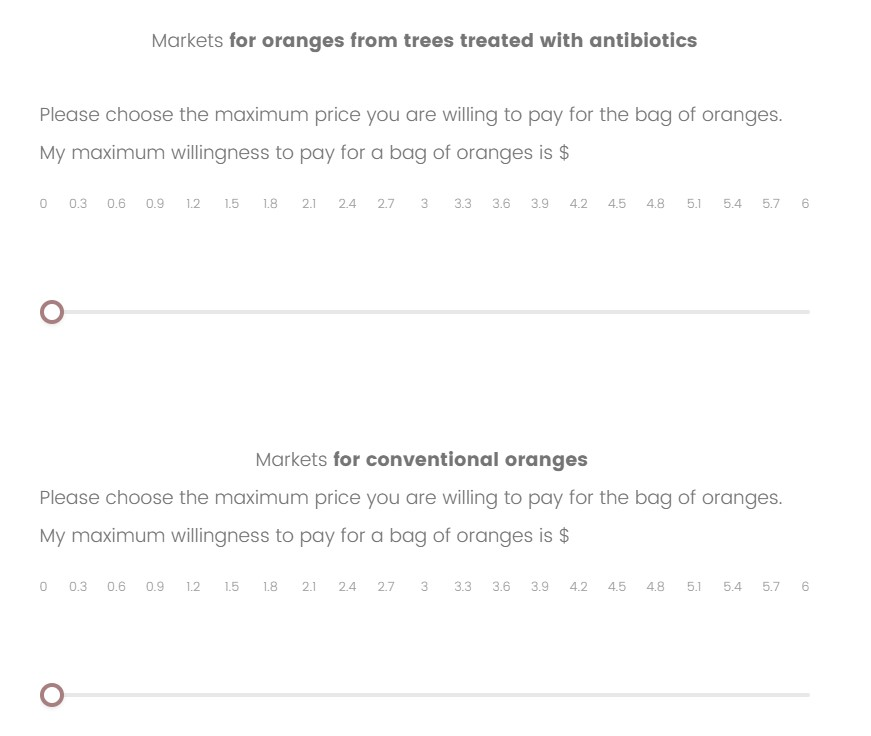
\includegraphics[width=0.8\linewidth]{BDM_market.jpg}

\end{figure}

\clearpage

\definecolor{navyblue}{RGB}{0, 0, 128}

\subsubsection*{Instructions (continued)}
Let me give you an example: Assume that you bid \textbf{\$3.00}, and the fixed price is \textcolor{cyan}{\$2.80}, then you win the orange and only pay \textcolor{cyan}{\$2.80}. If, however, your price was lower than the fixed price, then you do not buy the orange.  

You should offer the maximum price you are willing to pay for the orange; there are no advantages to strategic behavior in this task. Your best strategy is to determine your personal value for the orange and offer that price.  

\vspace{0.3cm}

\textbf{Why is it my best strategy to bid the maximum price I’d be willing to pay?}  

If I truly value the orange at \textbf{\$3.00}, however instead of bidding \textcolor{orange}{\$3.00}, I bid \textcolor{orange}{\$2.60}, and the fixed price is \textcolor{cyan}{\$2.80}, then I lose the opportunity to purchase the oranges. However, had I bid my true valuation I would have won and paid only \textcolor{cyan}{\$2.80} for an orange I think is worth \textbf{\$3.00}.  

Now what if I offer more? Let’s say that I truly valued the orange at \textbf{\$3.00} and I bid \textcolor{orange}{\$5.00}, and the fixed price ended up being \textcolor{orange}{\$4.40}. Then I win, I will have to pay \textcolor{cyan}{\$4.40} for an item I value at \textbf{\$3.00}.  

\vspace{0.5cm} 

When you have understood the instructions, please proceed to the next page.  


\clearpage


\subsubsection*{Instructions continued}


\textbf{Example 1}: If the card you own can be redeemed for a bonus of \$6.00, you bid \$3.00 and the fixed price is \$2.40, you have a higher bid than the fixed price. You buy the item, and you pay the fixed price (\$2.40), plus your balance is (\$6.00 - \$2.40 = \$3.60) and you get the product which will be shipped to your specified mailing address using priority shipping.
\vspace{0.5cm}


\textbf{Example 2}: If the card you own can be redeemed for a bonus of \$6.00, your bid is \$3.00 and the fixed price is \$4.00, you have a bid lower than the fixed price. You do not buy the item, and you receive your bonus of \$6.00.

\vspace{0.5cm}

When you have understood the instructions, please proceed to the next page.
\clearpage


\subsubsection*{Comprehension test}
Note: All following questions will provide simple explanations if the subject indicates or types the wrong answer(correct answer is in bold).

\vspace{0.5cm}

True or False? The fixed price will be a known number to me before I make a decision.  

• True  \par
\textbf{• False}\par  

\vspace{0.5cm}


\vspace{0.5cm}



True or False? My best strategy is to bid the maximum I'd be willing to pay.  

\textbf{• True}  \par
• False 

\vspace{0.5cm}

If I value both oranges at \$5.00:

\textbf{a) Although the value of my card is less than \$10.00, I can bid \$5.00 in each market. However, only one of these bids will be binding.}  

b) I can only bid in one market since the value of my card is less than \$10.00.  

\vspace{0.5cm}

If the card you own could be redeemed for a bonus of \$6.00, your bid was \$4.00 and the fixed price was \$2.4, what would have been your final outcome?  

\textbf{a) I pay \$2.40 for the orange, so my balance is \$6 - \$2.40 = \$3.60 } 

b) The value of my card is \$6.00, since I cannot buy the orange  

c) I pay \$4.00 for the orange, so my balance is \$6.00 - \$4.00 = \$2.00  

\vspace{0.5cm}

If the card you own could be redeemed for a bonus of \$6.00, your bid is \$3.40 and the fixed price is \$4.00, what would be your final outcome?  

d) I pay \$4.00 for the orange, so my balance is \$6.00 - \$4.00 = \$2.00  

\textbf{e) The value of my card is \$6.00, since I cannot buy the orange } 

f) I pay \$3.4 for the orange, so my balance is \$6.00 - \$3.40 = \$2.60  

\vspace{0.5cm}

\subsubsection*{\textbf{Instructions (continued)}}

You have successfully completed the comprehension test, and you will now begin Task 1.\par

\vspace{0.5cm}
 Please click next when you are ready to proceed.

Now, we will go to the main tasks. 

\textbf{Please remember this decision is hypothetical and you will not earn money or a bag of oranges.}

\clearpage

\subsubsection*{\centering \textbf{Round 1 \& 2}}

\begin{figure}[H]
    \centering
    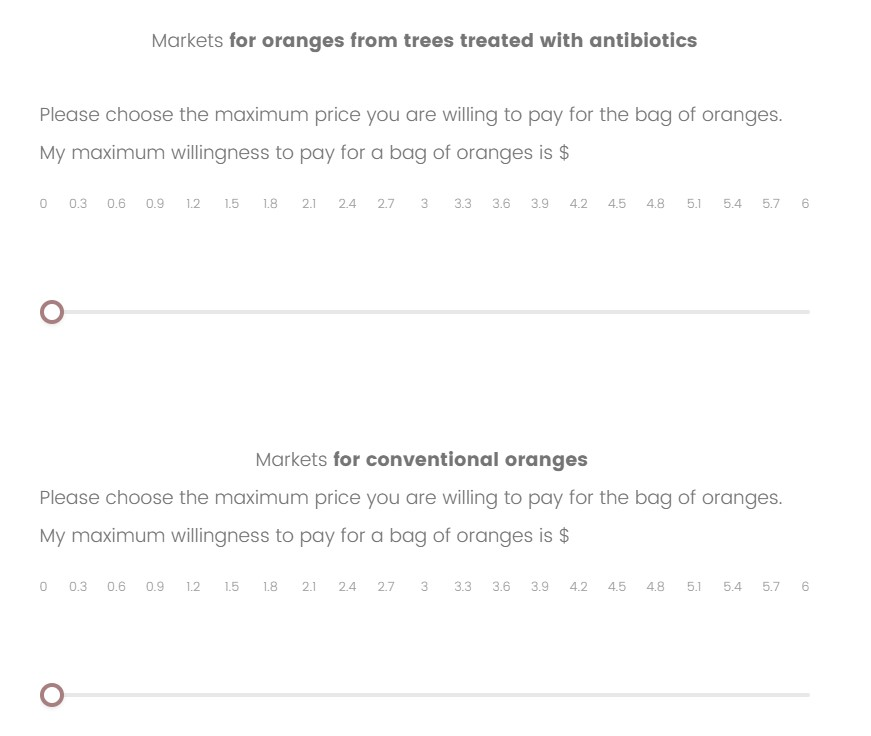
\includegraphics[width=0.8\linewidth]{BDM_market.jpg}
    \caption{}
    \label{fig:BDM_market}
\end{figure}

\clearpage

\subsubsection*{\textbf{Instructions (continued)}}
On the next page, you will see a video. \textbf{Please ensure your speakers or headphones are connected and the volume is set properly.} Next you will see a video that provides information about a disease Watch the video carefully in a quiet, distraction-free environment, as it is essential for the study.
\vspace{0.5cm}
Click on the video to watch it.

\href{https://www.youtube.com/watch?v=_AqMBjB0ChM}{video}
\clearpage


 \subsubsection*{\centering Round 3}


\begin{figure}[H]
    \centering
    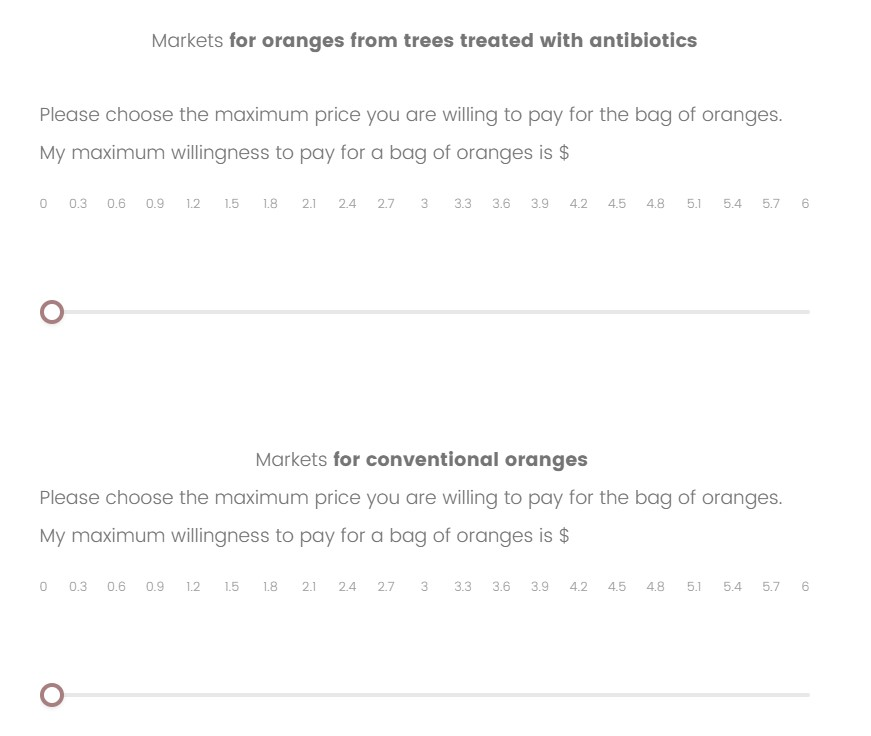
\includegraphics[width=\linewidth]{BDM_market.jpg}
    \caption{}
    \label{fig:BDM_market}
\end{figure}

\clearpage



\subsection{BDM Real}


\subsubsection*{\textbf{Instructions (continued)}}


For this study you will receive a fixed fee of \$2 and you can earn additional compensation in cash and/or citrus products based on your decisions and chance, so please pay attention to the instructions.
 
You will complete 3 Tasks that involve real money, so please pay attention to the instructions. There is a 10\% chance that your decisions will be selected for payment. After completing the 3 tasks, the computer will draw a random number between 1 and 10. If the random number is equal to 1, you will receive the payoff as described below. However, if the random number is between 2 and 10, your decision will not yield additional earnings, and you will receive just the \$2. If you are selected for payment, one of the three tasks will be randomly selected to be added to your compensation.

 Since there is a chance that your decision will end up affecting your earnings, it is in your best interest to respond carefully to each task. If your compensation includes a food product (oranges), the product will be shipped to your specified address *free of charge* via priority mail as long as you provide us with a valid mailing address. You will receive more details about this procedure below.

\clearpage

\subsubsection*{\textbf{Instructions (continued)}}

In this study, you will complete 3 Tasks and a survey.
For each task, you will be endowed with a card with a value of \$6.00. You can use the funds in the card to purchase a bag of oranges (3.2 lbs – approximately 6-8 oranges) in two distinct markets. Any remaining funds in the card that you don’t spend on the oranges will be added to your earnings on top of your \$2.00 participation fee if you are selected for payment.



In one market, the oranges are from trees treated with antibiotics by injection to the *tree’s trunks* (not directly in the orange fruits) to prevent yield and fruit quality losses caused by a disease called citrus greening. The other market is conventional oranges, not from trees treated with antibiotics, but using a combination of pesticides and cultural practices.


You can use the funds in your card to bid on one of the markets or both. Your bid will be compared to an unrelated fixed price that is equally likely to be a number between $0.00 and $6.00. If your bid is higher than the fixed price, you will purchase the item. But here is the interesting part, in this case, you do not pay the price you offer, instead you pay the fixed offer. If your bid is lower than the fixed price, you do not buy the orange and you do not pay anything. 

 

\textbf{Please remember this decision is real and you may earn money or any bag of oranges.}

 

 \clearpage

\subsubsection*{\textbf{Instructions (continued)}}

From that point, the instructions are the same as hypothetical, with a different reminder as shown below;

 Now, we will go to the main tasks.


\textbf{Please remember this decision is real and you may earn money or any bag of oranges.}

 \clearpage

 \subsection{GSO Hypothetical}
 \subsubsection*{\textbf{Instructions (continued)}}

For this study, we will explore your preferences for oranges. You will only receive a participation fee of \$2.00. In the next screen you will be presented with a hypothetical scenario. Note that the scenario is hypothetical, but we ask you to make your decisions as if you were in a real market using real money. Although we will describe the rules of the procedure shortly as if it actually involves money, you will not actually have to pay anything, and we will not ship any products to you. However, we do want you to treat it as if it was real. That is, although you will not receive a bag of oranges and you will not actually have to pay anything, we still want you to formulate your bid thinking what you would do if you had to do it for real. You will receive more details about this procedure below.


\clearpage

\subsubsection*{\textbf{Instructions (continued)}}

In this study, you will complete 3 Tasks and a survey.

For each task, you will be endowed with a card with a value of \$6.00. You can use the funds in the card to purchase a bag of oranges (3.2 lbs – approximately 6-8 oranges) in two distinct markets. Any remaining funds in the card that you don’t spend on the oranges will be added to your earnings on top of your \$2.00 participation fee if you are selected for payment.

In one market, the oranges are treated with antibiotics by injection to the *tree’s trunks* (not directly in the orange fruits) to prevent yield and fruit quality losses caused by a disease called citrus greening. The other market is conventional oranges, not treated with antibiotics, but using a combination of pesticides and cultural practices.

You can use the funds in your card to purchase from one of the markets or both.

 
\textbf{Please remember this decision is hypothetical and you will not earn money or any bag of oranges.}

\clearpage

\subsubsection*{\textbf{Instructions (continued)}}

 In each market, offer prices will be displayed on the screen, and you will make choices over several periods. For every period, you can click “Try to Buy” if you are willing to buy the bag of oranges at the corresponding offer price or click “Not Buy” if you are not willing to buy at that offer price.
The computer has already randomly chosen the \textbf{market price} at which it will accept to sell the bag of oranges to you. That price is drawn between \$0.00 and \$6.00 and is equally likely.

In the first period, the offer price starts at \textcolor{orange}{\$0.00 }and will increase by \$0.20 after every period. The task ends when the price on the screen increases to the \textbf{market price} that the computer chose to sell the bag of oranges.
At every other price, whether you choose “Try to Buy” or “Not Buy”, you will go to the next period and again choose between “Try to Buy” or “Not Buy”.
The task will continue until the offer price reaches the market price the computer chose to try to sell the bag of oranges to you. At that price:

\begin{enumerate}
    \item If you choose “Try to Buy”, you receive the market price, and task ends.
    \item If you choose “Not Buy” you will not be able to buy the bag of oranges and task ends.
\end{enumerate}


For example, let’s say you are in Period 1, when the offer price is \$0.00. If the computer tries to sell you the bag of oranges at that price, and you click “Try to Buy”, you will get the bag of oranges at the current price \$0.00. If instead you clicked “Not Buy”, you will not be able to buy the bag of oranges. However, if the computer does not try to sell you the bag of oranges at that price, you will go to the next period.

\clearpage



\subsubsection*{\textbf{Instructions (continued)}}


Here is a practice screen to familiarize yourself with the buttons or with the way you choose to buy or not buy. Your responses here will not count toward the main study.
Please keep making choices until the buttons turn red, that is when then the market is over.

\begin{figure}[H]
    \centering
    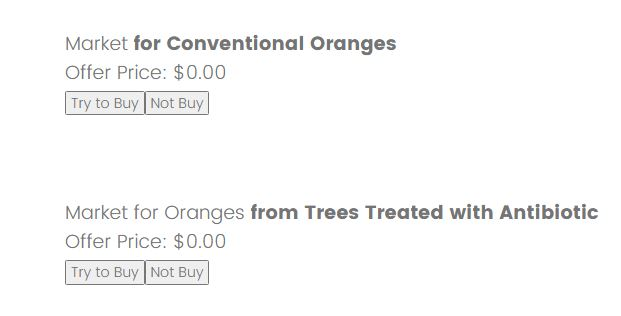
\includegraphics[width=0.8\linewidth]{GSO.JPG}
    
    \label{fig:GSO}
\end{figure}

\clearpage


\subsubsection*{\textbf{Instructions (continued)}}

\textbf{Example 1}

Suppose the maximum amount \textbf{Person X} is willing to pay for the bag of oranges is \textbf{\$3.00}. The first offer price starts at \textcolor{orange}{\$0.00}. Since Person X is willing to purchase the bag of oranges for \textcolor{orange}{\$0.00} (because Person X is willing to pay up to \$3.00), then He/ She would click “Try to Buy” at that offer price.

Suppose the randomly drawn \textbf{market price} from \$0.00 to \$6 is \$2.00 (you will not be able to see it), since the offer price is lower than the market price, Person X would not be able to buy the bag of oranges when selecting “Try to Buy”. He/ She will proceed to the next period where offer price will be \textcolor{orange}{\$0.20}.
Since Person X is willing to purchase the bag of oranges at \$0.20, He/ She would select “Try to Buy”. Once again, the offer price will be compared to the market price. Since the randomly drawn market price in our example was \$2.00, Person X would not buy the bag oranges and He/ She will proceed to the next offer price of \textcolor{orange}{\$0.40}.


This process will continue until the offer price is \textcolor{orange}{\$2.00}. When the offer price is \textcolor{orange}{\$2.00}, Person X chooses “try to buy” and since the market price is \textcolor{cyan}{\$2.00} a transaction will occur at that time. Note that Person X maximum willingness to pay for the bag of oranges was \textbf{\$3.00}, but the market price randomly generated by the computer was \textcolor{cyan}{\$2.00}. So, if selected for payment, Person X would purchase the bag of oranges and receive them via priority shipping to their designated mailing address and the remaining \$4.00 on their card will be added to their compensation.



Please proceed to the next page for another example.
\clearpage

\subsubsection*{\textbf{Instructions (continued)}}

Example 2

Suppose the maximum amount \textbf{Person X} is willing to pay for the bag of oranges is \textbf{\$3.00}. The first offer price starts at \textcolor{orange}{\$0.00}. Since Person X is willing to purchase the bag of oranges for \textcolor{orange}{\$0.00} (because Person X is willing to pay up to \$3.00), then He/ She would click “Try to Buy” at that offer price.

Suppose the randomly drawn market price from \$0.00 to \$6.00 is \textcolor{cyan}{\$4.00} (you will not be able to see it), since the offer price is lower than the market price, Person X would not be able to buy the bag of oranges when selecting “Try to Buy”. He/ She will proceed to the next period where offer price will be \textcolor{orange}{\$0.20}.

Since Person X is willing to purchase the bag of oranges at \textcolor{orange}{\$0.20}, He/ She would select “Try to Buy”. Once again, the offer price will be compared to the market price. Since the randomly drawn market price in our example was \textcolor{cyan}{\$4.00}, Person X would not buy the bag oranges, and He/ She will proceed to the next offer price of \textcolor{orange}{\$0.40}.


This process will continue until the offer price is \textcolor{orange}{\$3.00}.  However, in the next round, the offer price will be \textcolor{orange}{\$3.20}. When the offer price is \textcolor{orange}{\$3.20}, Person X would click “Not buy”. When clicking “Not buy”, she will go to the next round and will continue to click “Not Buy” until task ends and will not be able to buy the bag of oranges. In this example, task ends when the offer price reaches \textcolor{cyan}{\$4.00}. Person X will click “Not Buy” at this price and will not be able to buy the bag of oranges.
\vspace{0.5cm}

When you have understood the instructions, please proceed to the next page.
\clearpage

\subsubsection*{Comprehension test}

Select which statement below is the most correct

\begin{itemize}
    \item The price increases by \$0.20 in each subsequent period 
    \item The value of your card does not change
    \item \textbf{Both answers are true}
\end{itemize}

\vspace{0.5cm}

What will happen to your reward if you try to buy when the fixed price is \$4.40, and the computer accepts your price?

\begin{itemize}
    \item I will get \$6, which is the value of my card
    \item \textbf{I will pay the oranges at \$4.40, plus get my balance of \$6.00-4.40=\$1.60}
    \item It is random
\end{itemize}

\vspace{0.5cm}


If the price of oranges in both markets is \$5.00 at a given period, can I try to buy both oranges in both markets?

\begin{itemize}
    \item No, you can’t because your card is worth \$6, it exceeds your endowment.
    \item \textbf{Yes, you can, however if the computer accepts both prices, only one decision will be randomly binding for realization.}
\end{itemize}

\vspace{0.5cm}

If Person' X maximum willingness to pay for the orange is \$3.00, S/He would switch from "Try to Buy" to "Not Buy" at \$3.20.

\begin{itemize}
    \item \textbf{Then Person X will continue to click "Not Buy" until the market ends}
    
    \item Person X should try to switch back and forth to "Try to Buy" and "Not Buy"
    \item None of these answers is correct
\end{itemize}

\clearpage



\subsubsection*{Comprehension test (continued)}

You have successfully completed the comprehension test, and you will now begin Task 1.

 Please click next when you are ready to proceed.

 Now, we will go to the main tasks. 
 
 \textbf{Please remember this decision is hypothetical and you will not earn money or any bag of oranges.}


\clearpage

 \subsubsection*{Round 1\& 2}


 \begin{figure}[H]
    \centering
    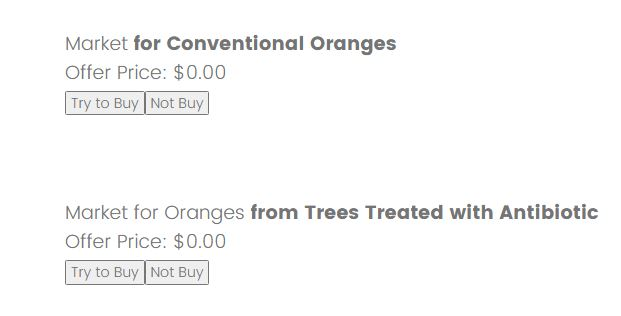
\includegraphics[width=0.8\linewidth]{GSO.JPG}
    
    \label{fig:GSO}
\end{figure}

 \vspace{0.5cm}


On the next page, you will see a video. \textbf{Please ensure your speakers or headphones are connected and the volume is set properly.} Next you will see a video that provides information about a disease Watch the video carefully in a quiet, distraction-free environment, as it is essential for the study.
\vspace{0.5cm}
Click on the video to watch it.

\href{https://www.youtube.com/watch?v=_AqMBjB0ChM}{video}
\clearpage


 \subsubsection*{Round 3}



\begin{figure}[H]
    \centering
    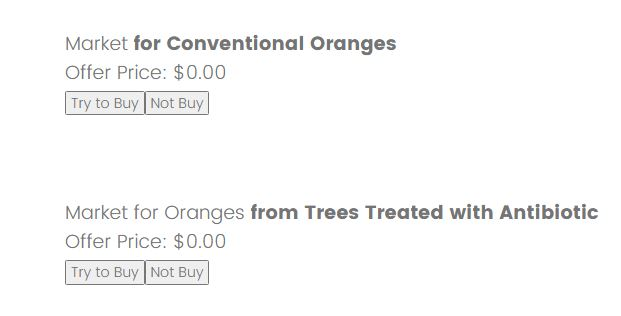
\includegraphics[width=\linewidth]{GSO.JPG}
    \caption{}
    \label{fig:Appendix_GSO_game}
\end{figure}
 

\clearpage



\subsection{GSO Real}

\subsubsection*{Instructions}

For this study you will receive a fixed fee of \$2.00 and you can earn additional compensation in cash and/or citrus products based on your decisions and chance, so please pay attention to the instructions.
 
You will complete 3 Tasks that involve real money, so please pay attention to the instructions. There is a 10\% chance that your decisions will be selected for payment. After completing the 3 tasks, the computer will draw a random number between 1 and 10. If the random number is equal to 1, you will receive the payoff as described below.
However, if the random number is between 2 and 10, your decision will not yield additional earnings, and you will receive just the \$2.00. If you are selected for payment, one of the three tasks will be randomly selected to be added to your compensation.

\textbf{Since there is a chance that your decision will end up affecting your earnings, it is in your best interest to respond carefully to each task}. If your compensation includes a food product (oranges), the product \textbf{will be shipped to your specified address *free of charge* via priority mail} as long as you provide us with a valid mailing address. You will receive more details about this procedure below.


\clearpage

\subsubsection*{Instructions (continued)}

In this study, you will complete 3 Tasks and a survey.

For each task, you will be endowed with a card with a value of \$6.00. You can use the funds in the card to purchase a bag of oranges (3.2 lbs – approximately 6-8 oranges) in two distinct markets. Any remaining funds in the card that you don’t spend on the oranges will be added to your earnings on top of your \$2.00 participation fee if you are selected for payment.

In one market, the oranges are from trees treated with antibiotics by injection to the *tree’s trunks* (not directly in the orange fruits) to prevent yield and fruit quality losses caused by a disease called citrus greening. The other market is conventional oranges, not from trees treated with antibiotics, but using a combination of pesticides and cultural practices.

You can use the funds in your card to purchase from one of the markets or both.

\textbf{ Please remember this decision is real and you may earn money or any bag of oranges.}

\clearpage

\subsubsection*{Instructions (continued)}

 From that point, the instructions are the same as hypothetical, with a different reminder as shown below;

 Now, we will go to the main tasks.
\vspace{0.5cm}

\textbf{Please remember this decision is real and you may earn money or any bag of oranges.}


 \clearpage

\section{Background on citrus greening}
\label{AppedixOrange}
 The United States, which was once the world leader in citrus production, producing 50\% of the world's citrus in 1970, has experienced a decrease in its global share to 25\% in 2000, then to 5\% in 2023 \citep{munch_us_2023} . As a result of this staggering decline in domestic production, the country relies more on imports from countries such as Mexico and Chile. The recent decline in citrus production over the past 15 years in the US is mainly a result of a bacterial disease known as "Huanglongbing" (HLB) or citrus greening. This disease was first discovered in Florida in 2005, it accounts; for the infection of 80\% of citrus plants in Florida \citep{li2020citrus} and increases  production cost of farmers \citep{roka2009citrus} . This disease, caused by the bacteria "Liberibacter asiaticus", results in chlorosis of the foliage, reduction of absorption of nutrients and yield, and death of citrus trees within 3 years \citep{bove_huanglongbing_2006}. The citrus greening also affects the marketability of the citrus by distorting its size, visual feature, ripening (partial or not at all), and flavor \citep{farnsworth_potential_2024}. Orange juice made from infected citrus fruit has a higher concentration of limonin and nomilin leading to a sour taste of citrus juice \citep{paula2018active}. 

Previously, to address HLB, systematic tree removal was recommended to combat HLB. However, this approach was not sustainable for multiple reasons. First, symptomatic citrus trees could still produce some marketable fruit, making immediate tree removal financially cumbersome for farmers. Second, replacing an infected tree with a new one incurs high costs for farmers, as it takes several years before new trees begin to bear fruit.  Finally, the effect of tree removal is undermined by the external cost. If some farmers decide not to remove infected trees, the disease contributes to spreading, negating the effort of others \citep{farnsworth_potential_2024}. Recently, the administration of antibiotics through trunk injections has been investigated and found to be a promising method to control HLB \citep{li_precision_2022}. \citet{archer_trunk_2023} corroborates this discovery by showing that the administration of oxytetracyclin through injection into the trunk of orange trees results in a decrease in fruit loss before harvest, as well as an improvement in fruit output, size, and juice quality.

Antibiotics administration has been applied for decades in cattle. However, according to \citet{hosain_antimicrobial_2021}, it has drawbacks on human health; it accounts for 80\% of antimicrobial resistance (AMR) in USA annually, and AMR affects 2.8 million people, causing more than 35.000 deaths \citep{cdc2019antibiotic}.  The use of antibiotics can effectively help to manage the dissemination of HLB, thus protecting citrus trees. Consequently, this can be advantageous to citrus farmers and all other stakeholders involved in the citrus industry at the state level in Florida. Antibiotics can help decrease Florida's reliance on imported citrus, thus preventing the probable extinction of citrus at the state level. This is undesirable for those who enjoy Florida citrus fruits and juice, as well as those who prefer locally sourced products. Ultimately, it can help preserve the superior taste of juice, preventing the occurrence of a bitter flavor that may arise from citrus fruits obtained from infected trees. The use of antibiotics also comes with some challenges. First, it may cause health hazards (AMR) if relevant policy is not reinforced on dosage and injection timing. Second, it may leave  residues in wastewater that could lead to soil pollution. In light of this dilemma, it directs our attention to determining how consumers will respond to the use of antibiotics in the production of citrus fruit since the success of such techniques depends on the acceptance of consumers, which also depends on the way information is communicated. Although the use of antibiotics in livestock has been extensively studied, it is unfortunate that the literature is silent about consumers’ preference for foods treated with antibiotics; hence, we propose filling this gap.

\clearpage










\section{Tables for main results}

\begin{table}[htbp]
\centering
\footnotesize
\caption{Standardized Differences comparing participants included vs excluded in the study}
\label{tab:Incomplete}
\begin{threeparttable}
\begin{tabular}{llccc}
\toprule
\textbf{Variable} & \textbf{Category} & \textbf{Include} & \textbf{Exclude} & \textbf{Std. Diff} \\
\midrule
\multirow{2}{*}{Ethnicity} & Non-White & 413 (34.90\%) & 345 (31.10\%) & 0.08 \\
                           & White     & 771 (65.10\%) & 766 (68.90\%) & \\
\midrule
\multirow{3}{*}{Income Category} & Low income    & 537 (46.3\%) & 535 (50.90\%) & 0.14 \\
                                 & Middle income & 519 (44.70\%) & 397 (37.80\%) & \\
                                 & High income   & 104 (9\%)  & 119 (11.30\%) & \\
\midrule
\multirow{4}{*}{Region} & Northeast & 200 (16.90\%) & 196 (17.70\%) & 0.07 \\
                        & Midwest   & 265 (22.40\%) & 259 (23.40\%) & \\
                        & South     & 464 (39.30\%) & 397 (35.80\%) & \\
                        & West      & 252 (21.30\%) & 257 (23.20\%) & \\
\midrule
\multirow{2}{*}{Gender} & Male   & 573 (49.10\%) & 523 (48.20\%) & 0.02 \\
                        & Female & 593 (50.90\%) & 562 (51.80\%) & \\
\midrule
\multirow{2}{*}{Education} & No Bachelor & 751 (63.40\%) & 701 (63.10\%) & 0.007 \\
                           & Bachelor    &  433   (36.60\%)        &   410 (36.90\%)          &  \\
\midrule
\multirow{2}{*}{Children} & Children     & 405 (35\%) & 207 (19.80\%) & 0.34 \\
                          & No Children  & 753 (65\%) & 839 (80.20\%) & \\
\midrule
\multirow{2}{*}{Marital Status} & Married     & 419 (35.40\%) & 365 (32.90\%) & 0.05 \\
                                & Not Married &   765 (64.60\%)          &    746 (67.10\%)         & \\
\midrule
Age  & & 46 (16.53) & 53.32 (17.96) & -0.424 \\
\bottomrule
\end{tabular}
\begin{tablenotes}
\footnotesize
\item Notes: Standardized differences are calculated between those included and excluded in the study. Number not in parentheses represent number of participants, those in parentheses represent proportions for categorical variables and standard deviations for continuous ones.
\end{tablenotes}
\end{threeparttable}
\end{table}

\clearpage


    \begin{table}[htbp!]
\centering
\caption{Standardized Differences Across Variables}
\label{tab:Appendix_std_diff_table}
\resizebox{\textwidth}{!}{%
\begin{tabular}{lcccccc}
\hl& \multicolumn{3}{c}{\textbf{GSO Real vs.}} & \multicolumn{2}{c}{\textbf{BDM Real vs.}} & \textbf{GSO Hypo vs.} \\
\cmidrule(lr){2-4} \cmidrule(lr){5-6} \cmidrule(lr){7-7}
\textbf{Variable}        & \textbf{BDM Real} & \textbf{GSO Hypo} & \textbf{BDM Hypo} & \textbf{GSO Hypo} & \textbf{BDM Hypo} & \textbf{BDM Hypo} \\
\hline

Hispanic        & 0.0884        & 0.0114        & 0.0630        & 0.0770        & 0.0254        & 0.0516 \\
Income\_category        & 0.1704        & 0.0462        & 0.1440        & 0.1498        & 0.0431        & 0.1153 \\
Region  & 0.1326        & 0.1861        & 0.1918        & 0.1064        & 0.0779        & 0.0850 \\
Gender  & 0.0834        & 0.0178        & 0.0228        & 0.0927        & 0.0627        & 0.0379 \\
Education       & 0.2267        & 0.1748        & 0.1342        & 0.0514        & 0.0919        & 0.0404 \\
children        & 0.0584        & 0.0128        & 0.0869        & 0.0456        & 0.0284        & 0.0740 \\
Marital status  & 0.0952        & 0.0322        & 0.0437        & 0.1274        & 0.0514        & 0.0759 \\
Age     & -0.0160       & 0.0753        & -0.0557       & 0.0883        & -0.0380       & -0.1285 \\

\hline \hline
\end{tabular}}
\begin{tablenotes}
\item Notes: GSO stands for the Game Structure Obvious mechanism treatment; BDM stands for the Becker-DeGroot-Marschak mechanism treatment; Real and Hypothetical stand for the real and hypothetical incentives treatments, respectively.
\end{tablenotes}
\end{table}
  
 
\clearpage


        % Right column for the second table

            \begin{table}[htbp]
                \centering
                \caption{Descriptive Statistics by Treatment 
                (excluding excluding MS (R1: 14.2\%, R2, 9.6\%, R3: 3.6\%)
)}
                \label{tab:Appendix_descrip_2}
                \resizebox{1\textwidth}{!}{%
                \begin{tabular}{lccc}
                \hline \hline
                \textbf{Treatment}    & \textbf{N (including MSB)}       & \textbf{Mean (USD)}  & \textbf{Standard Deviation} \\
                \hline
                GSO Real           & 288                        & 3.50       & 1.20                  \\
                BDM Real            & 313                        & 3.48       & 1.36                \\
                GSO Hypothetical     & 295                     & 3.63      & 1.16                   \\
                BDM Hypothetical      & 320                  & 3.44       & 1.30                    \\
                \midrule
                \textbf{Total}         & \textbf{1,216}              & \textbf{3.48} & \textbf{1.26}         \\
                \hline\hline
              
                \end{tabular}}
\begin{tablenotes}
            \footnotesize
            
            \item Notes: GSO stands for the Game Structure Obvious mechanism treatment; BDM stands for the Becker-DeGroot-Marschak mechanism treatment; Real and Hypo stand for the real and hypothetical incentives treatments, respectively.
           % \item $\times$: interaction
           % \item MS: A dummy variable for MS
           % \item GSOMSB: A dummy variable for being GSO and with MS
        \end{tablenotes}
            \end{table}
       
     
\clearpage
  











 \begin{table}[H]
                \centering
                \caption{Interval Model of Consumer WTP for Oranges (Baseline: BDM Real)}
                \label{tab:interval_regression}
                \resizebox{\textwidth}{!}{% Scale table to fit the column width
    \begin{tabular}{l*{4}{cc}}
    \hline \hline
            &\multicolumn{2}{c}{WTP}    &\multicolumn{2}{c}{WTP (control 1)}    &\multicolumn{2}{c}{WTP (control 2)}    &\multicolumn{2}{c}{WTP (control 3)}    \\
    \hline        
Constant    &       3.476\sym{***}&     (0.050)&       3.476\sym{***}&     (0.050)&       3.210\sym{***}&     (0.138)&       3.197\sym{***}&     (0.138)\\
GSO         &       0.042         &     (0.080)&                     &            &       0.027         &     (0.080)&                     &            \\
Hypothetical&      -0.016         &     (0.070)&      -0.016         &     (0.070)&      -0.030         &     (0.070)&      -0.030         &     (0.070)\\
GSOXHypothetical&       0.258\sym{**} &     (0.110)&                     &            &       0.311\sym{***}&     (0.113)&                     &            \\
GSOnoMSB    &                     &            &       0.029         &     (0.082)&                     &            &       0.011         &     (0.082)\\
GSOnoMSBXHypothetical&                     &            &       0.228\sym{**} &     (0.113)&                     &            &       0.280\sym{**} &     (0.116)\\
GSOMSB      &                     &            &       0.228         &     (0.211)&                     &            &       0.252         &     (0.215)\\
GSOMSBXHypothetical&                     &            &       0.517\sym{**} &     (0.261)&                     &            &       0.571\sym{**} &     (0.266)\\
Round2      &                     &            &                     &            &       0.049\sym{*}  &     (0.027)&       0.052\sym{*}  &     (0.027)\\
Round3      &                     &            &                     &            &       0.092\sym{***}&     (0.030)&       0.102\sym{***}&     (0.030)\\
White       &                     &            &                     &            &      -0.045         &     (0.064)&      -0.043         &     (0.064)\\
Middle Income&                     &            &                     &            &      -0.079         &     (0.064)&      -0.081         &     (0.064)\\
High Income &                     &            &                     &            &      -0.015         &     (0.115)&      -0.013         &     (0.115)\\
Midwest     &                     &            &                     &            &      -0.176\sym{**} &     (0.087)&      -0.181\sym{**} &     (0.086)\\
South       &                     &            &                     &            &      -0.079         &     (0.078)&      -0.080         &     (0.078)\\
West        &                     &            &                     &            &      -0.112         &     (0.085)&      -0.118         &     (0.085)\\
Female      &                     &            &                     &            &       0.032         &     (0.054)&       0.037         &     (0.054)\\
Bachelor    &                     &            &                     &            &      -0.048         &     (0.061)&      -0.046         &     (0.060)\\
No Children &                     &            &                     &            &       0.019         &     (0.068)&       0.024         &     (0.068)\\
Married     &                     &            &                     &            &      -0.061         &     (0.061)&      -0.063         &     (0.061)\\
Age         &                     &            &                     &            &       0.009\sym{***}&     (0.002)&       0.009\sym{***}&     (0.002)\\
\hline
$\sigma_u $    &       1.091\sym{***}&     (0.019)&       1.088\sym{***}&     (0.019)&       1.080\sym{***}&     (0.019)&       1.077\sym{***}&     (0.019)\\
$\sigma_e $     &       0.846\sym{***}&     (0.020)&       0.846\sym{***}&     (0.020)&       0.845\sym{***}&     (0.019)&       0.844\sym{***}&     (0.019)\\
\hline
\(n\) (observations)      &        7104         &            &        7104         &            &        6828         &            &        6828         &            \\

\(N \) (subjects)      &        1184         &            &        1184         &            &        1138         &            &        1138         &            \\
\hline \hline
\end{tabular}
}




\begin{tablenotes}
            \footnotesize
           \item Bootstrap Standard errors (1000 times) in parentheses. * p$<$0.1, ** p$<$0.05, *** p$<$0.01.
            \item \textit{Note:} $\sigma_u$ and $\sigma_e$ denote the standard deviations of the random intercept and residual error, respectively.
            \item Notes: GSO stands for the Game Structure Obvious mechanism treatment; BDM stands for the Becker-DeGroot-Marschak mechanism treatment; Real and Hypo stand for the real and hypothetical incentives treatments, respectively.
           \item $\times$: interaction
           \item GSOnoMSB: A dummy variable for being GSO and no MS.
           \item GSOMSB: A dummy variable for being GSO and with MS.
           \item Baseline: BDM Real. represents the baseline treatment group of the regression analysis.
        \end{tablenotes}
            \end{table}

\clearpage








\begin{table}[H]
        \centering
      \caption{Comparison of Willingness to Pay by Instruction Comprehension Scores (demean test score) }
        \label{tab:MSB_interval_regression_Score_overall}
       \resizebox{0.7\textwidth}{!}{% Scale table to fit the column width
      \begin{tabular}{l*{1}{cc}}
      \hline \hline
            &\multicolumn{2}{c}{WTP (BDM Real: baseline)}    \\
            \hline
Constant    &       3.096\sym{***}&     (0.140)\\
GSO         &       0.085         &     (0.083)\\
Hypothetical&       0.125         &     (0.078)\\
GSO$\times$Hypothetical&       0.162         &     (0.118)\\
Test\_score  &       0.052\sym{**} &     (0.023)\\
GSO$\times$Test\_score&      -0.157\sym{***}&     (0.038)\\
Hypothetical$\times$Test\_score&       0.017         &     (0.036)\\
GSO$\times$Hypothetical$\times$Test\_score&       0.006         &     (0.055)\\
Round2      &       0.049\sym{*}  &     (0.027)\\
Round3      &       0.092\sym{***}&     (0.030)\\
White       &      -0.043         &     (0.065)\\
Middle Income&      -0.056         &     (0.064)\\
High Income &       0.005         &     (0.115)\\
Midwest     &      -0.154\sym{*}  &     (0.086)\\
South       &      -0.075         &     (0.077)\\
West        &      -0.103         &     (0.085)\\
Female      &       0.033         &     (0.053)\\
Bachelor    &      -0.040         &     (0.061)\\
No Children &       0.030         &     (0.068)\\
Married     &      -0.039         &     (0.061)\\
Age         &       0.009\sym{***}&     (0.002)\\
\hline
$\sigma_u $    &       1.069\sym{***}&     (0.020)\\
$\sigma_e $     &       0.845\sym{***}&     (0.019)\\
\hline
\(n\) (observations)      &        6828         &            \\
\(N\) (subjects)       &        1138         &            \\
\hline \hline
\end{tabular}
}

\begin{tablenotes}
            \footnotesize
            \item Bootstrap Standard errors (1000 times) in parentheses. * p$<$0.1, ** p$<$0.05, *** p$<$0.01.
            \item \textit{Note:} $\sigma_u$ and $\sigma_e$ denote the standard deviations of the random intercept and residual error, respectively.
            \item Notes: GSO stands for the Game Structure Obvious mechanism treatment; BDM stands for the Becker-DeGroot-Marschak mechanism treatment; Real and Hypo stand for the real and hypothetical incentives treatments, respectively.
           \item $\times$: Interaction.
           \item Baseline: BDM Real. represents the baseline treatment group for the right hand-side \\
        \end{tablenotes}
\end{table}



\clearpage






\begin{table}[H]
        \centering
      \caption{Comparison of Willingness to Pay by Complexity Scores (demean complexity) }
        \label{tab:Complexity}
       \resizebox{0.7\textwidth}{!}{% Scale table to fit the column width
      \begin{tabular}{l*{1}{cc}}
      \hline \hline
            &\multicolumn{2}{c}{WTP (BDM Real: baseline)}    \\
            \hline
Constant    &       3.218\sym{***}&     (0.139)\\
GSO         &       0.029         &     (0.081)\\
Hypothetical&      -0.019         &     (0.072)\\
GSO$\times$Hypothetical&       0.308\sym{***}&     (0.114)\\
Complexity  &       0.013         &     (0.048)\\
GSO$\times$Complex\_score&       0.021         &     (0.084)\\
Hypothetical$\times$Complex\_score&      -0.089         &     (0.069)\\
GSO$\times$Hypothetical$\times$Complex\_score&       0.161         &     (0.109)\\
Round2      &       0.049\sym{*}  &     (0.027)\\
Round3      &       0.092\sym{***}&     (0.030)\\
White       &      -0.043         &     (0.065)\\
Middle Income&      -0.083         &     (0.065)\\
High Income &      -0.023         &     (0.115)\\
Midwest     &      -0.179\sym{**} &     (0.087)\\
South       &      -0.085         &     (0.078)\\
West        &      -0.114         &     (0.085)\\
Female      &       0.027         &     (0.054)\\
Bachelor    &      -0.042         &     (0.061)\\
No Children &       0.023         &     (0.068)\\
Married     &      -0.066         &     (0.061)\\
Age         &       0.009\sym{***}&     (0.002)\\
\hline
$\sigma_u $    &       1.078\sym{***}&     (0.019)\\
$\sigma_e$     &       0.845\sym{***}&     (0.019)\\

\hline
\(n\) (observations)      &        6828         &            \\
\(N\) (subjects)       &        1138         &            \\
\hline \hline
\end{tabular}
}

\begin{tablenotes}
            \footnotesize
            \item Bootstrap Standard errors (1000 times) in parentheses. * p$<$0.1, ** p$<$0.05, *** p$<$0.01.
            \item \textit{Note:} $\sigma_u$ and $\sigma_e$ denote the standard deviations of the random intercept and residual error, respectively.
            \item Notes: GSO stands for the Game Structure Obvious mechanism treatment; BDM stands for the Becker-DeGroot-Marschak mechanism treatment; Real and Hypo stand for the real and hypothetical incentives treatments, respectively.
           \item $\times$: Interaction.
           \item Baseline: BDM Real. represents the baseline treatment group for the right hand-side \\
        \end{tablenotes}
\end{table}



\clearpage





 \begin{table}[H]
        \centering
        \caption{Comparison of Willingness to Pay (social desirability)}
        \label{tab:interval_regression_socialdesirability_BDM}
        \resizebox{0.8\textwidth}{!}{% Scale table to fit the column width
        \begin{tabular}{l*{2}{cc}}
        \hline \hline
            &\multicolumn{2}{c}{WTP: GSO (Yes)}    &\multicolumn{2}{c}{WTP: BDM (Yes)}    \\
            \hline
Constant    &       3.483\sym{***}&     (0.388)&       3.466\sym{***}&     (0.182)\\
Hypothetical&       0.345\sym{**} &     (0.167)&       0.164\sym{*}  &     (0.096)\\
AfterInformation&       0.135         &     (0.116)&       0.167         &     (0.115)\\
HypotheticalXAfterInformation&      -0.230         &     (0.162)&      -0.120         &     (0.163)\\
White       &      -0.200         &     (0.187)&      -0.213\sym{**} &     (0.085)\\
Middle Income&      -0.425\sym{**} &     (0.190)&       0.110         &     (0.094)\\
High Income &       0.162         &     (0.254)&       0.129         &     (0.158)\\
Midwest     &      -0.037         &     (0.265)&      -0.242\sym{*}  &     (0.135)\\
South       &       0.128         &     (0.245)&      -0.063         &     (0.117)\\
West        &       0.126         &     (0.287)&      -0.336\sym{***}&     (0.123)\\
Female      &       0.048         &     (0.156)&       0.178\sym{**} &     (0.080)\\
Bachelor    &       0.040         &     (0.180)&       0.030         &     (0.095)\\
No Children &       0.220         &     (0.173)&       0.164\sym{*}  &     (0.097)\\
Married     &       0.011         &     (0.181)&      -0.255\sym{***}&     (0.089)\\
Age         &       0.003         &     (0.005)&       0.006\sym{**} &     (0.003)\\
\hline
$\sigma_u $    &       0.942\sym{***}&     (0.057)&                     &            \\
$\sigma_e $    &       0.898\sym{***}&     (0.057)&                     &            \\
\hline
\(n\) (observations)       &         984         &            &        1176         &            \\
\(N \) (subjects)      &        164         &            &        196         &            \\
\hline \hline
\multicolumn{5}{l}{\footnotesize Standard errors in parentheses. * p$<$0.1, ** p$<$0.05 *** p$<$0.01}\\
\end{tabular}
}

\begin{tablenotes}
            \footnotesize
            \item Bootstrap Standard errors (1000 times) in parentheses. * p$<$0.1, ** p$<$0.05, *** p$<$0.01.
            \item \textit{Note:} $\sigma_u$ and $\sigma_e$ denote the standard deviations of the random intercept and residual error, respectively.
            \item Notes: GSO stands for the Game Structure Obvious mechanism treatment; BDM stands for the Becker-DeGroot-Marschak mechanism treatment; Real and Hypo stand for the real and hypothetical incentives treatments, respectively.
           \item $\times$: Interaction.
           \item Baseline: BDM Real. represents the baseline treatment group for the right hand-side \\
           GSO Real represents the Baseline treatment group for the left-hand side.
           \item Yes: Represents the sample of participants who mention they would support antibiotics treatment for citrus.
        \end{tablenotes}
\end{table}

\clearpage







 \begin{table}[H]
        \centering
        \caption{Comparison of Willingness to Pay by Type of Oranges}
        \label{tab:Orange_socialdesirability_BDM}
        \resizebox{0.7\textwidth}{!}{% Scale table to fit the column width
        \begin{tabular}{l*{2}{cc}}
        \hline \hline
            &\multicolumn{2}{c}{WTP: GSO }    &\multicolumn{2}{c}{WTP: BDM }    \\
            \hline
Constant    &       3.442\sym{***}&     (0.210)&       3.046\sym{***}&     (0.122)\\
Hypothetical&       0.323\sym{***}&     (0.102)&      -0.054         &     (0.060)\\
AntibioticsOranges&       0.020         &     (0.066)&       0.069         &     (0.064)\\
HypotheticalXAntibioticsOranges&      -0.074         &     (0.095)&       0.057         &     (0.089)\\
Round2      &       0.026         &     (0.050)&       0.059         &     (0.054)\\
Round3      &       0.025         &     (0.055)&       0.120\sym{**} &     (0.055)\\
White       &      -0.071         &     (0.099)&      -0.023         &     (0.051)\\
Middle Income&      -0.070         &     (0.100)&      -0.102\sym{*}  &     (0.053)\\
High Income &       0.347\sym{*}  &     (0.182)&      -0.253\sym{***}&     (0.094)\\
Midwest     &      -0.086         &     (0.134)&      -0.251\sym{***}&     (0.074)\\
South       &      -0.015         &     (0.127)&      -0.136\sym{**} &     (0.067)\\
West        &      -0.066         &     (0.137)&      -0.141\sym{*}  &     (0.074)\\
Female      &      -0.089         &     (0.087)&       0.106\sym{**} &     (0.046)\\
Bachelor    &      -0.238\sym{**} &     (0.100)&       0.120\sym{**} &     (0.051)\\
No Children &       0.188\sym{*}  &     (0.106)&      -0.131\sym{**} &     (0.053)\\
Married     &      -0.215\sym{**} &     (0.098)&       0.064         &     (0.051)\\
Age         &       0.006\sym{*}  &     (0.003)&       0.011\sym{***}&     (0.001)\\
\hline
$\sigma_u $    &       1.140\sym{***}&     (0.032)&                     &            \\
$\sigma_e $     &       0.834\sym{***}&     (0.036)&                     &            \\
\hline
\(n\) (observations)    &        3288         &            &        3540         &            \\
\(N\) (subjects)      &        538         &            &        590         &            \\
\hline \hline
\multicolumn{5}{l}{\footnotesize Standard errors in parentheses. * p$<$0.1, ** p$<$0.05 *** p$<$0.01}\\
\end{tabular}
}

\begin{tablenotes}
            \footnotesize
           \item Bootstrap Standard errors (1000 times) in parentheses. * p$<$0.1, ** p$<$0.05, *** p$<$0.01.
            \item \textit{Note:} $\sigma_u$ and $\sigma_e$ denote the standard deviations of the random intercept and residual error, respectively.
            \item Notes: GSO stands for the Game Structure Obvious mechanism treatment; BDM stands for the Becker-DeGroot-Marschak mechanism treatment; Real and Hypo stand for the real and hypothetical incentives treatments, respectively.
           \item $\times$: Interaction.
           \item Baseline: BDM Real. represents the baseline treatment group for the right hand-side \\
           GSO Real represents the Baseline treatment group for the left-hand side.
           \item Antibiotics oranges: A dummy variable equal to 1 for oranges from trees treated with antibiotics as compared to conventional oranges.
        \end{tablenotes}
\end{table}







\begin{table}[H]
        \centering
        \caption{Comparison of Willingness to Pay by Round for GSO}
        \label{tab:interval_regression_RounbyRound}
    \resizebox{0.8\textwidth}{!}{%
    \begin{tabular}{l*{1}{cc}}
    \hline\hline
    & Coefficient & (Bootstrap SE) \\
    \hline
    Constant & 3.206\sym{***} & (0.139) \\
    GSO & 0.013 & (0.093) \\
    Hypothetical & -0.045 & (0.079) \\
    GSO$\times$Hypothetical & 0.422\sym{***} & (0.134) \\
    Round2 & 0.075 & (0.048) \\
    Round3 & 0.081 & (0.053) \\
    GSO$\times$Round2 & 0.018 & (0.084) \\
    GSO$\times$Round3 & 0.019 & (0.092) \\
    Hypothetical $\times$ Round 2 & -0.032 & (0.067) \\
    Hypothetical$\times$Round 3 & 0.076 & (0.075) \\
    GSO$\times$Hypothetical$\times$Round2 & -0.103 & (0.117) \\
    GSO$\times$Hypothetical$\times$Round3 & -0.227\sym{*} & (0.133) \\
    White & -0.045 & (0.064) \\
    Middle Income & -0.079 & (0.064) \\
    High Income & -0.015 & (0.115) \\
    Midwest & -0.175\sym{**} & (0.087) \\
    South & -0.079 & (0.078) \\
    West & -0.112 & (0.085) \\
    Female & 0.032 & (0.054) \\
    Bachelor & -0.047 & (0.061) \\
    No Children & 0.019 & (0.068) \\
    Not Married & -0.063 & (0.061) \\
    Age & 0.009\sym{***} & (0.002) \\
    \hline
    $\sigma_u$ & 1.080\sym{***} & (0.019) \\
   $\sigma_e$ & 0.845\sym{***} & (0.019) \\
    \hline
\(n \) (observations)      &        6828                 \\
\(N \) (subjects)      &        1138           \\
\hline\hline
    
    \end{tabular}
    }



\begin{tablenotes}
            \footnotesize
            \item Bootstrap Standard errors (1000 times) in parentheses. * p$<$0.1, ** p$<$0.05, *** p$<$0.01.
            \item \textit{Note:} $\sigma_u$ and $\sigma_e$ denote the standard deviations of the random intercept and residual error, respectively.
            \item Notes: GSO stands for the Game Structure Obvious mechanism treatment; BDM stands for the Becker-DeGroot-Marschak mechanism treatment; Real and Hypo stand for the real and hypothetical incentives treatments, respectively.
           \item $\times$: Interaction.
           \item GSOMSB: A dummy variable for being GSO and with MS.
           \item Baseline: BDM Real. represents the baseline treatment group for the right hand-side.
           GSO Real represents the Baseline treatment group for the left-hand side.
        \end{tablenotes}
\end{table}











\clearpage



\begin{table}[H]
        \centering
        \caption{Time spent and hypothetical bias in GSO}        \label{tab:Time_spent}
       \resizebox{0.7\textwidth}{!}{% Scale table to fit the column width
     \begin{tabular}{l*{1}{cc}}
\hline\hline
            &\multicolumn{2}{c}{(1)}           \\
            &\multicolumn{2}{c}{Time spent}      \\
\hline
Constant    &       7.856\sym{***}&     (0.119)\\
Hypothetical&      -0.172\sym{**} &     (0.079)\\
Round2      &      -0.472\sym{***}&     (0.079)\\
Round3      &      -0.531\sym{***}&     (0.078)\\
HypotheticalXRound2&       0.034         &     (0.110)\\
HypotheticalXRound3&      -0.020         &     (0.111)\\
White       &      -0.046         &     (0.049)\\
Middle Income&      -0.068         &     (0.052)\\
High Income &      -0.049         &     (0.100)\\
Midwest     &      -0.104         &     (0.073)\\
South       &      -0.110         &     (0.067)\\
West        &      -0.005         &     (0.077)\\
Female      &      -0.023         &     (0.046)\\
Bachelor    &      -0.022         &     (0.053)\\
No Children &      -0.122\sym{**} &     (0.052)\\
Married     &       0.100\sym{*}  &     (0.053)\\
Age         &       0.015\sym{***}&     (0.002)\\
\hline
\(N\)       &        3288         &            \\
\hline\hline
\multicolumn{3}{l}{\footnotesize Standard errors in parentheses. * p$<$0.1, ** p$<$0.05 *** p$<$0.01}\\
\end{tabular}
}


\begin{tablenotes}
            \footnotesize
          \item Bootstrap Standard errors (1000 times) in parentheses. * p$<$0.1, ** p$<$0.05, *** p$<$0.01.
            \item Notes: GSO stands for the Game Structure Obvious mechanism treatment; Real and Hypo stand for the real and hypothetical incentives treatments, respectively.
           \item $\times$: interaction
           \item Baseline: GSO Real represents the Baseline treatment group 
        \end{tablenotes}
\end{table}

\clearpage





\begin{table}[H]
        \centering
      \caption{Comparison of Willingness to Pay by time (logarithm) }
        \label{tab:Time_hypobias}
       \resizebox{0.60\textwidth}{!}{% Scale table to fit the column width
      \begin{tabular}{l*{1}{cc}}
      \hline \hline
            &\multicolumn{2}{c}{WTP (BDM Real: baseline)}    \\
            \hline
Constant    &       1.319\sym{***}&     (0.388)\\
GSO         &       7.127\sym{***}&     (0.608)\\
Hypothetical&       0.917\sym{*}  &     (0.504)\\
GSO$\times$\Hypothetical&      -0.312         &     (0.808)\\
Round2      &       0.090         &     (0.327)\\
Round3      &       0.478         &     (0.408)\\
GSO$\times$Round2&      -0.269         &     (0.545)\\
GSO$\times$Round3  &      -0.479         &     (0.613)\\
Hypothetical$\times$Round2&       0.633         &     (0.414)\\
Hypothetical$\times$Round3&       0.072         &     (0.489)\\
GSO$\times$\Hypothetica$\times$Round2&      -0.983         &     (0.782)\\
GSO$\times$Hypothetica$\times$Round3&      -0.792         &     (0.852)\\
ln\_time     &       0.183\sym{***}&     (0.038)\\
GSO$\times$ln\_time&      -0.853\sym{***}&     (0.071)\\
Hypothetical$\times$ln\_time&      -0.100\sym{*}  &     (0.051)\\
GSO$\times$Hypothetical$\times$ln\_time&       0.050         &     (0.095)\\
ln\_time$\times$Round2&      -0.002         &     (0.033)\\
ln\_time$\times$Round3&      -0.041         &     (0.041)\\
GSO$\times$ln\_time$\times$Round2&      -0.003         &     (0.065)\\
GSO$\times$ln\_time$\times$Round3&       0.009         &     (0.072)\\
Hypothetical$\times$ln\_time$\times$Round2&      -0.069\sym{*}  &     (0.042)\\
Hypothetical$\times$ln\_time$\times$Round3&       0.001         &     (0.049)\\
GSO$\times$Hypothetical$\times$ln\_time$\times$Round2&       0.104         &     (0.097)\\
GSO$\times$Hypothetical$\times$ln\_time$\times$Round3&       0.062         &     (0.104)\\
White       &      -0.044         &     (0.058)\\
Middle Income&      -0.090         &     (0.057)\\
High Income &      -0.074         &     (0.108)\\
Midwest     &      -0.162\sym{**} &     (0.079)\\
South       &      -0.099         &     (0.072)\\
West        &      -0.121         &     (0.080)\\
Female      &       0.022         &     (0.049)\\
Bachelor    &      -0.010         &     (0.055)\\
No Children &      -0.001         &     (0.061)\\
Married     &      -0.037         &     (0.055)\\
Age         &       0.012\sym{***}&     (0.002)\\
$\sigma\_u $    &       0.961\sym{***}&     (0.019)\\
$\sigma\_u $     &       0.812\sym{***}&     (0.019)\\
\hline

\(n\) (observations)      &        6828         &            \\
\(N\) (subjects)       &        1138         &            \\
\hline \hline
\end{tabular}
}

\begin{tablenotes}
            \footnotesize
            \item Bootstrap Standard errors (1000 times) in parentheses. * p$<$0.1, ** p$<$0.05, *** p$<$0.01.
            \item \textit{Note:} $\sigma_u$ and $\sigma_e$ denote the standard deviations of the random intercept and residual error, respectively.
            \item Notes: GSO stands for the Game Structure Obvious mechanism treatment; BDM stands for the Becker-DeGroot-Marschak mechanism treatment; Real and Hypo stand for the real and hypothetical incentives treatments, respectively.
           \item $\times$: Interaction.
           \item Baseline: BDM Real. represents the baseline treatment group for the right hand-side.
           \item Time: Demeaned time spent per increment.
        \end{tablenotes}
\end{table}




\clearpage
%%%%%%%%%%%%%%%%%%%%%%%%%%%%%%%%%%%%%%%%%%%%%%%%%%%%%%%%%%%%%%%%%%%%%%%%%%%%%%%%%%%%%%%%%%%%%%%%%%%%%%%%%%%%%%%%%%%%%%%%%%%%%%a%%%%%%
\section{Appendix sections excluding MSB}




 \begin{table}[H]
                \centering
                \caption{Interval Model of Consumer WTP for Oranges (Baseline: BDM Real)}
                \label{tab:MSB_interval_regression_multiple_comaparisons}
                \resizebox{0.85\textwidth}{!}{% Scale table to fit the column width
             \begin{tabular}{l*{3}{cc}}
             \hline \hline
            &\multicolumn{2}{c}{WTP     (full sample)}    &\multicolumn{2}{c}{WTP (exclude MSB)}    &\multicolumn{2}{c}{WTP (only MSB)}    \\

Constant    &       3.210\sym{***}&     (0.138)&       3.205\sym{***}&     (0.139)&       3.185\sym{***}&     (0.170)\\
GSO         &       0.027         &     (0.080)&       0.006         &     (0.081)&       0.466\sym{***}&     (0.164)\\
Hypothetical&      -0.030         &     (0.070)&      -0.030         &     (0.070)&      -0.026         &     (0.070)\\
GSO$\times$Hypothetical&       0.311\sym{***}&     (0.113)&       0.273\sym{**} &     (0.115)&       0.326         &     (0.204)\\
Round2      &       0.049\sym{*}  &     (0.027)&       0.043         &     (0.027)&       0.067\sym{**} &     (0.033)\\
Round3      &       0.092\sym{***}&     (0.030)&       0.096\sym{***}&     (0.030)&       0.127\sym{***}&     (0.037)\\
White       &      -0.045         &     (0.064)&      -0.049         &     (0.065)&      -0.026         &     (0.078)\\
Middle Income&      -0.079         &     (0.064)&      -0.104         &     (0.065)&      -0.039         &     (0.078)\\
High Income &      -0.015         &     (0.115)&      -0.018         &     (0.115)&      -0.205         &     (0.149)\\
Midwest     &      -0.176\sym{**} &     (0.087)&      -0.203\sym{**} &     (0.088)&      -0.241\sym{**} &     (0.100)\\
South       &      -0.079         &     (0.078)&      -0.079         &     (0.079)&      -0.169\sym{*}  &     (0.094)\\
West        &      -0.112         &     (0.085)&      -0.110         &     (0.086)&      -0.185\sym{*}  &     (0.101)\\
Female      &       0.032         &     (0.054)&       0.039         &     (0.054)&       0.100         &     (0.068)\\
Bachelor    &      -0.048         &     (0.061)&      -0.053         &     (0.062)&       0.094         &     (0.073)\\
No Children &       0.019         &     (0.068)&       0.010         &     (0.068)&      -0.047         &     (0.080)\\
Married     &      -0.061         &     (0.061)&      -0.078         &     (0.062)&       0.049         &     (0.077)\\
Age         &       0.009\sym{***}&     (0.002)&       0.010\sym{***}&     (0.002)&       0.008\sym{***}&     (0.002)\\
\hline
$\sigma_u$     &       1.080\sym{***}&     (0.019)&       1.086\sym{***}&     (0.020)&       1.011\sym{***}&     (0.027)\\
$\sigma_e$     &       0.845\sym{***}&     (0.019)&       0.838\sym{***}&     (0.020)&       0.845\sym{***}&     (0.024)\\

\hline
\(n\) (observations)      &        6828         &            &        6531         &            &        3837         &            \\

\(N\) (subjects)       &        1138         &            &       NA         &            &        NA       &            \\
\hline\hline
\end{tabular}
}


\begin{tablenotes}
            \footnotesize
            \item Bootstrap Standard errors (1000 times) in parentheses. * p$<$0.1, ** p$<$0.05, *** p$<$0.01.
            \item \textit{Note:} $\sigma_u$ and $\sigma_e$ denote the standard deviations of the random intercept and residual error, respectively.
            \item Notes: GSO stands for the Game Structure Obvious mechanism treatment; BDM stands for the Becker-DeGroot-Marschak mechanism treatment; Real and Hypo stand for the real and hypothetical incentives treatments, respectively.
           \item $\times$: Interaction.
           \item GSOMSB: A dummy variable for being GSO and with MS.
           \item GSOMSB: A dummy variable for being GSO and with no MS.
           \item Baseline: BDM Real, represents the baseline treatment group for the right hand-side.
           GSO Real represents the Baseline treatment group for the left-hand side.
        \end{tablenotes}

\end{table}

\clearpage




\begin{table}[H]
        \centering
        \caption{Factor predicting MSB  in the GSO}    
        \label{tab:MSB_predictor1}
       \resizebox{0.7\textwidth}{!}{% Scale table to fit the column width
      \begin{tabular}{l*{1}{cc}}
      \hline \hline
            &\multicolumn{2}{c}{Multiple switching}    \\
            \hline
Constant    &      -1.044\sym{***}&     (0.400)\\
test\_score  &      -0.144\sym{***}&     (0.030)\\
Certainty     &      -0.259\sym{***}&     (0.065)\\
Complexity\_score&       0.264\sym{***}&     (0.055)\\
White       &       0.029         &     (0.135)\\
Middle Income&      -0.037         &     (0.147)\\
High Income &      -0.882\sym{***}&     (0.327)\\
Midwest     &       0.157         &     (0.211)\\
South       &       0.175         &     (0.190)\\
West        &       0.530\sym{**} &     (0.208)\\
Female      &      -0.452\sym{***}&     (0.130)\\
Bachelor    &       0.057         &     (0.150)\\
No Children &      -0.350\sym{**} &     (0.144)\\
Married     &      -0.011         &     (0.146)\\
Age         &      -0.002         &     (0.005)\\
\hline
\(n\) (observations)      &        3288         &            \\
\(N\) (subjects)       &        548         &            \\
\hline \hline
\end{tabular}
}

\begin{tablenotes}
            \footnotesize
         \item Bootstrap Standard errors (1000 times) in parentheses. * p$<$0.1, ** p$<$0.05, *** p$<$0.01.
            \item \textit{Note:} Certainty: a variable that varies from 1 to 5 representing how certain participants were about their valuation.
            \item Complexity\_score: Perceived complexity of the mechanism.
        \end{tablenotes}
\end{table}







\clearpage


\begin{table}[H]
        \centering
        \caption{Comparison of Willingness to Pay by MS in GSO}        \label{tab:MSB_interval_regression_MSB}
       \resizebox{0.7\textwidth}{!}{% Scale table to fit the column width
      \begin{tabular}{l*{1}{cc}}
      \hline \hline
            &\multicolumn{2}{c}{WTP}    \\
            \hline
Constant    &       3.406\sym{***}&     (0.209)\\
Hypothetical&       0.256\sym{***}&     (0.094)\\
GSOMSB      &       0.213         &     (0.219)\\
Hypothetical$\times$GSOMSB&       0.302         &     (0.267)\\
Round2      &       0.035         &     (0.050)\\
Round3      &       0.055         &     (0.055)\\
White       &      -0.068         &     (0.098)\\
Middle Income&      -0.073         &     (0.099)\\
High Income &       0.354\sym{*}  &     (0.182)\\
Midwest     &      -0.100         &     (0.133)\\
South       &      -0.020         &     (0.126)\\
West        &      -0.082         &     (0.135)\\
Female      &      -0.077         &     (0.087)\\
Bachelor    &      -0.235\sym{**} &     (0.100)\\
No Children &       0.197\sym{*}  &     (0.105)\\
Married     &      -0.216\sym{**} &     (0.097)\\
Age         &       0.006\sym{**} &     (0.003)\\
\hline
$\sigma_u $    &       1.133\sym{***}&     (0.032)\\
$\sigma_e $     &       0.831\sym{***}&     (0.036)\\

\hline
\(n\) (observations)       &        3288         &            \\
\(N\) (subjects)       &        548         &            \\
\hline \hline
\end{tabular}
}

\begin{tablenotes}
            \footnotesize
            \item Bootstrap Standard errors (1000 times) in parentheses. * p$<$0.1, ** p$<$0.05, *** p$<$0.01.
            \item \textit{Note:} $\sigma_u$ and $\sigma_e$ denote the standard deviations of the random intercept and residual error, respectively.
            \item Notes: GSO stands for the Game Structure Obvious mechanism treatment; Real and Hypo stand for the real and hypothetical incentives treatments, respectively.
           \item Baseline: GSO Real represents the Baseline treatment group for the left-hand side.
        \end{tablenotes}
\end{table}





\clearpage





















\end{document}